\documentclass{article}
\usepackage{nips14submit_e,times}

\title{Pure Exploration of Combinatorial Bandits}
\author{Shouyuan Chen}
\date{\today}
%%%%%%%%%%%%%%%%%%%%%%%%%%%%%%%%%%%%%%%%%%%%%%%%%%%%%%%%%%%%%

% Change "article" to "report" to get rid of page number on title page
\usepackage{amsmath,amsfonts,amsthm,amssymb}
\usepackage{setspace}
\usepackage{Tabbing}
\usepackage{fancyhdr}
\usepackage{lastpage} 
\usepackage{extramarks}
\usepackage{chngpage}
\usepackage{soul,color}
\usepackage{graphicx,float,wrapfig}
\usepackage{afterpage}
\usepackage{abstract}
\usepackage[colorlinks=true,linkcolor=blue,citecolor=blue]{hyperref}
\usepackage[numbers]{natbib}
\usepackage{algpseudocode}
\usepackage{algorithm}
\usepackage{xspace}
\usepackage{subcaption}
\usepackage{theoremref}
\usepackage{thmtools}
\usepackage{thm-restate}
\usepackage{cleveref}

%\usepackage{titling}


\allowdisplaybreaks

%%%%%%%%%%%%%%%%%%%%%%%%%%%%%%%%%%%%%%%%%%%%%%%%%%%%%%%%%%%%%
% Some tools
\newcommand{\junk}[1]{}

%\newtheorem{define}{Definition}
%\newtheorem{example}{Example}
%\newtheorem{lemma}{Lemma}
%\newtheorem{corollary}{Corollary}
%\newtheorem{theorem}{Theorem}

\declaretheorem{theorem}
\declaretheorem{lemma}
\declaretheorem{corollary}
\declaretheorem{define}
\declaretheorem[name=Fact,Refname={Fact,Facts}]{fact}

\declaretheorem{example}
%\declaretheoremstyle[bodyfont=normalfont]{mystyle}
%\declaretheorem[style=mystyle]{example}

%\def\ttdefault{blg}

\newcommand{\Algorithm}{{\small \textsf{CGapExp}}\xspace}
\newcommand{\AlgorithmPAC}{{\small \textsf{CGapExpPAC}}\xspace}
\newcommand{\AlgorithmBud}{{\small \textsf{CGapKill}}\xspace}
\newcommand{\Problem}{{\small \textsf{ExpCMAB}}\xspace}
\newcommand{\Rew}{\varphi}
\newcommand{\E}{\mathbb E}

\newcommand{\M}{\mathcal M}
\newcommand{\mmatch}{\mathcal M_{\mathsf{MATCH}}}
\newcommand{\mtop}{\mathcal M_{\mathsf{TOP}m}}
\newcommand{\mbandit}{\mathcal M_{\mathsf{BANDIT}m}}

\newcommand{\diff}{\mathsf{diff}}
\newcommand{\diffvalid}{\prec}
\newcommand{\B}{\mathcal B}
\newcommand{\C}{\mathcal C}
\newcommand{\del}{\backslash}

\newcommand{\RR}{\mathbb R}

%\newcommand{\vec}[1]{\mathbf #1}

\newcommand{\Bopt}{\mathcal B_{\mathsf{opt}}}
\newcommand{\Bmatch}{\mathcal B_{\mathsf{MATCH}}}
\newcommand{\Btop}{\mathcal B_{\mathsf{TOP}m}}
\newcommand{\Bbandit}{\mathcal B_{\mathsf{BANDIT}m}}

\DeclareMathOperator{\supp}{supp}

\DeclareMathOperator{\rank}{width}
\DeclareMathOperator{\rad}{rad}
\DeclareMathOperator{\decomp}{decomp}
\DeclareMathOperator*{\argmax}{arg\,max}
\DeclareMathOperator*{\argmin}{arg\,min}
\DeclareMathOperator{\Oracle}{Oracle}
\DeclareMathOperator{\COracle}{COracle}
\DeclareMathOperator{\Exchange}{Exchange}

\newcommand{\out}{\mathsf{Out}}
\newcommand{\barlog}{\tilde{\log}}

\let\Pr\undefined
\DeclareMathOperator{\Pr}{Pr}

\newcommand{\MultiIdent}{\textsc{TopK}\xspace}
\newcommand{\MultiBandit}{\textsc{MB}\xspace}
\newcommand{\Matroid}{\textsc{Matroid}\xspace}
\newcommand{\Match}{\textsc{Match}\xspace}
\newcommand{\Path}{\textsc{Path}\xspace}

\newcommand{\inn}[1]{\left\langle #1 \right\rangle}
\newcommand{\nor}[1]{\left\|#1\right\|}
\renewcommand{\vec}[1]{\boldsymbol{#1}}

\renewcommand{\odot}{\circ}

%%%%%%%%%%%%%%%%%%%%%%%%%%%%%%%%%%%%%%%%%%%%%%%%%%%%%%%%%%%%%

\begin{document}
\newpage

\maketitle

\begin{abstract}
We study the structured pure exploration problem in the stochastic multi-armed bandit setting.
In particular, we formulate the \Problem problem where a learner's objective is to identify the optimal set of arms from a collection of sets of arms which we called decision class.
The decision class could be a collection of size $k$ subsets, matchings, spanning trees or paths. 
The generality of decision classes allows \Problem to represent a rich class of structured pure exploration problems.
We present two algorithms for the \Problem problem: one for the fixed confidence setting and one for the fixed budget setting.
We prove problem-dependent upper bounds of our algorithms. 
Our analysis exploits the combinatorial structures of the decision classes and introduces a new analysis tool.
We also establish a general problem-dependent lower bound for the \Problem problem.
Our results show that the proposed algorithms achieve optimal sample complexity (within logarithmic factors) for many decision classes. 
In addition, when applying our results back to top-$K$ arms identification and multiple bandit best arms identification, we recover the best known upper bounds and settles two open conjectures on the lower bounds.


% objective is to identify the optimal set of arms from a collection of sets of arms called decision class.

\end{abstract}

\section{Introduction}

For more than fifty years, multi-armed bandit (MAB) has been a predominant model for characterizing the tradeoff between exploration and exploitation in decision-making problems. 
Although this kind of tradeoff is intrinsic in many tasks, some application domains prefer a dedicated exploration procedure in which the goal is to identify an optimal object among several candidates and the profit/cost incurred during exploration is irrelevant.
In light of these applications, the related learning problem, called pure exploration in MABs, has received much attention.
Recent results of pure exploration MABs have found potential applications in many domains including crowdsourcing, communication network and online advertising.

In many  of these application domains, a recurring problem is to identify an optimal object with certain \emph{combinatorial structures}. 
For example, a crowdsourcing application may want to find the best assignment from workers to tasks such that overall productivity of workers are maximized. 
A network routing system during an initialize phase may tries to build a spanning tree that minimizes the delay of links, or attempts to identify the shortest path between two sites.  
An online advertising system may be interested to find the best matching between ads and displaying slots. 
The literature of pure exploration MAB problems lacks a framework that encompasses these kinds of problems where the object of interest has a non-trivial combinatorial structure.  
Our paper contributes such a framework which accounts for general combinatorial structures, and develops a series of results, including algorithms, upper bounds and lower bounds.

In this paper, we formulate the Pure Exploration in Combinatorial Bandits (\Problem) problem.  
In an \Problem problem, a learner has a fixed set of arms and each arm is associated with an unknown reward distribution. 
The learner is also given a collection of sets of arms called \emph{decision class}. 
The objective is to find the optimal set of arms, which maximizes the sum of expected reward, from the given decision class. 
Over a sequence of rounds, the learner chooses an arm and observes a random reward sampled from the associated distribution. 
In the end, the learner is asked to output a member of the decision class which she believes to be optimal.


The \Problem framework represents a rich class of pure exploration problems.
The conventional pure exploration problem in MAB, where the objective is to find the single best arm, clearly fits into this framework, in which the decision class is the collection of all singletons. 
This framework also naturally encompasses several recent extensions, including the problem of finding the top $K$ arms (henceforth, \MultiIdent) \citep{kalyanakrishnan2010efficient,kalyanakrishnan2012pac,bubeck2013multiple,zhou2014optimal} and the problem of finding the best arms simultaneously from several disjoint sets of arms (henceforth, \MultiBandit) \citep{NIPS2011_4478,bubeck2013multiple}, by constructing proper decision classes. 
%The decision classes associated with these problems are relatively flat. 
Furthermore, this framework also covers many more interesting cases where the decision classes correspond to non-trivial combinatorial structures.
%By allowing general decision classes, this framework represents a rich class of pure exploration problems including many interesting cases where the decision classes correspond to non-trivial combinatorial structures.
%More interesting cases 
%Apart from these simple cases, the decision classes may correspond to non-trivial combinatorial structures. 
%Mo a substantially larger class of pure exploration problems.
For example, suppose that the arms represent the edges in a graph.
Then a decision class could be the set of all paths between two vertices, all spanning trees or all matchings of the graph. 
And, in these cases, the objectives of \Problem correspond to identifying the optimal paths, spanning trees and matchings, respectively.
As we have explained earlier, these kind of structured pure exploration problems admit applications in diverse domains.% including crowdsourcing, network routing and online advertising.
%Therefore, due to its generality, our framework admits applications in diverse domains including the examples we previously explained.

%More importantly, our framework covers a substantially larger class of pure exploration problems including many interesting cases where the decision classes correspond to non-trivial combinatorial structures. 
%For example, suppose that the arms represent the edges in a graph, then a decision class could be the set of all paths between two vertices, all spanning trees or all matchings of the graph. 
%As we have explained, exploring objects with these kind of structures may have applications 
%Therefore, by choosing different decision classes, our framework represents a rich class of pure exploration problems.

%Finding optimal objects from decision classes with non-trivial structures
The generality of \Problem framework raises several interesting challenges to the design and analysis of pure exploration algorithms. 
One challenge is that the arms with the largest mean rewards may not belong to the optimal set. For example, consider the case where the decision class is the set of all matchings in a bipartite graph.  
In this case, a matching consisting of edges with relatively small weights may turn out to be optimal.  
On the other hand, in many existing algorithms for pure exploration MABs, arms would no longer be considered once their expected reward are proven suboptimal during the learning process. 
Therefore, the design and analysis of algorithms for \Problem demands different techniques which take both rewards and structures into account.
\junk{
Before describing our results, we recall two common settings in pure exploration problems: fixed confidence and fixed budget. 
In the fixed confidence setting, the learner need to guarantee that she correctly identifies the optimal set with high probability while uses a small number of rounds(samples).  
In the fixed budget setting, the learner uses at most a fixed number of samples and she need to minimize her probability of error (identifies a suboptimal set).
}

\textbf{Our results.}
%In this paper, we develop a learning algorithm for the \Problem problem in the fixed confidence setting that supports a very wide range of decision classes, which is referred as Combinatorial Gap Exploration (\Algorithm) algorithm.%
We present Combinatorial Gap Exploration (\Algorithm) algorithm, a learning algorithm for the \Problem problem in the fixed confidence setting that supports a very wide range of decision classes. 
The proposed \Algorithm algorithm does not need to know anything about the details of the decision class's definition, as long as it has access to the decision class through a maximization oracle.
%Algorithm is an efficient and practical algorithm that works for a very wide range of decision classes. 
We prove a sample complexity bound of \Algorithm. 
The sample complexity bound depends on both expected reward and the structure of decision class. 
When specializing our result into \MultiIdent and \MultiBandit, we recover previous sample complexity bounds due to \citet{kalyanakrishnan2012pac} and \citet{gabillon2012best}.
% with a small improvement in the logarithmic factors. 
While for other decision classes in general, our result establishes the first sample complexity upper bound. 
Our analysis relies on a novel combinatorial construction called \emph{exchange class} which we believed may be of independent interest for other combinatorial optimization problems. 
We further show that \Algorithm can be easily extended to the fixed budget setting and PAC learning setting and we provide related theoretical guarantees.  

Moreover, we prove a problem-dependent sample complexity lower bound for the \Problem problem.  
Our lower bound shows that the sample complexity of the proposed \Algorithm algorithm is optimal (to within logarithmic factors) for a large class of decision classes, including \MultiIdent, \MultiBandit and the decision classes derived from matroids (e.g. spanning tree). 
Therefore our upper and lower bounds  provide a near full characterization of the sample complexity of these pure exploration problems. 
In addition, for general decision classes, our results find our the upper and lower bounds are within a relatively benign factor. 
To the best of our knowledge, there are few problem-dependent lower bounds known for pure exploration MABs besides the case of identifying the single best arm \citep{mannor2004sample,audibert2010best}.
We also notice that our result resolves the open conjectures of \citet{kalyanakrishnan2012pac} and \citet{bubeck2013multiple} on the sample complexity lower bounds of \MultiIdent and \MultiBandit problem.

In supplement to our main algorithm \Algorithm, we develop a parameter-free algorithm called Combinatorial Gap-based Elimination (\AlgorithmBud) algorithm, for the fixed budget setting. 
We prove a probability of error bound of the \AlgorithmBud algorithm. 
This bound can be shown to be equivalent to the sample complexity bound of \Algorithm within logarithmic factors, although the two algorithms are based on quite different techniques. 
Our analysis of \AlgorithmBud re-uses exchange classes as tools. 
This suggests that exchange class may be useful for the analysis of similar problems. 
In addition, when applying the algorithm to \MultiIdent and \MultiBandit, our bound recovers a recent result due to \citet{bubeck2013multiple}. 


\textbf{Notations.} 

\section{Problem Formulation}
%Let $\vec u \in \RR^{n}$ be a vector. 
% and $M\subseteq [n]$ be a set. 
%\textbf{\Problem: problem formulation.} 
In this section,  we formally define the \Problem problem.
Suppose that there are $n$ arms and the arms are numbered $1,2,\ldots,n$.
Assume that each arm $e\in[n]$ is associated with a reward distribution $\Rew_e$.
% and we let $w(e)=\E_{X\sim \Rew_e}[X]$ denote the expected reward. 
Let $\vec w = \big(w(1),\ldots, w(n)\big)^T$ denote the vector of expected rewards, where each entry $w(e)=\E_{X\sim \Rew_e}[X]$ denote the expected reward of arm $e$.
Following standard assumptions of stochastic MABs, we assume that all reward distributions are $R$-sub-Gaussian for some constant $R>0$. 
Formally, if $X$ is a random variable drawn according to $\Rew_e$, then, for all $t\in \RR$, one has $\mathbb E\big[\exp(tX-t\mathbb E[X])\big] \le \exp(R^2t^2/2)$ and $\mathbb E\big[\exp(t\mathbb E[X]-tX)\big] \le \exp(R^2t^2/2)$.
It is well known that all distributions that are supported on $[0,R]$ satisfy this property [].


We define a \emph{decision class} $\M \subseteq 2^{[n]}$ as a collection of sets of arms.
Let $M_*=\argmax_{M\in \M} w(M)$ denote the optimal set belonging to the decision class $\M$ which maximizes the sum of expected reward\footnote{For convenience, we will assume that $M_*$ is unique throughout the paper.}. 
A learner's objective is to identify $M_*$ from $\M$ by playing the following game.
%Let $\M\subseteq 2^{[n]}$ be the family of all feasible solutions to a combinatorial problem.
%Let $M_* = \argmax_{M\in \M} w(M)$ denote the optimal set of arms which max
%A learner wants to find the optimal solution of $\M$ which maximizes the expected reward $M_*=\argmax_{M\in \M} w(M)$ by playing the following game.
%The learning problem of pure exploration combinatorial bandit can be formalized as a game between a learner and a stochastic environment, where the learner's goal is to find the optimal solution to the combinatorial problem which maximizes the sum of expected reward $M_* = \argmax_{M\in \M} w(M)$.
At the beginning of the game, the decision class $\M$ is revealed to the learner while the reward distributions $\{\Rew_e\}_{e\in[n]}$ are unknown to the learner.
Then, the learner plays the game over a sequence of rounds;
on each round $t$, the learner pulls an arm $p_t\in [n]$ and observes a reward sampled from the associated reward distribution $\Rew_{p_t}$.
The game continues until certain stopping condition is satisfied.
%which will be specified later.
After the game finishes, the learner need to output a set $\out \in \M$.
%For the sake of simplicity, we shall assume that the optimal set $M_*$ is unique throughout the paper.

%Let $n$ denote the number of arms and suppose that the arms are numbered $1,2,\ldots,n$.

%We assume that all reward distributions are $R$-sub-Gaussian [].
%Notice that all distributions that are supported on $[0,R]$ are $R$-sub-Gaussian distributions [] and therefore our model subsumes the cases of bounded rewards.
%Let $w(e)=\E_{X\sim \Rew_e}[X]$ denote the expected reward of arm $e$ and let $\vec w = \big(w(1),\ldots,w(n)\big)^T$ denote the vector of expected rewards.
%In addition, for any set of arms $M\subseteq [n]$, we define $w(M) = \sum_{e\in M} w(e)$ as the sum of expected rewards of arms that belong to $M$.

%Notice that, if $\epsilon = 0$, then the learner is required to identify the optimal set, i.e. $\out = M_*$.



%\textbf{Fixed confidence and fixed budget.} 
We consider two different stopping conditions of the game, which are known as \emph{fixed confidence} setting and \emph{fixed budget} setting.
In the fixed confidence setting, the learner can stop the game at any point. 
The learner need to guarantee that $\Pr[\out = M_*] \ge 1-\delta$ for a given confidence parameter $\delta$.
%and her goal is to achieve a fixed confidence about the optimality of the returned set while uses a small number of pulls.
%Specifically, given a confidence parameter $\delta$, the learner 
The learner's performance is evaluated by her \emph{sample complexity}, i.e. the number of pulls used by the learner.
%Notice that the learner can stop the game at any point in this setting.
In the fixed budget setting, the game stops after a fixed number $T$ of rounds, where $T$ is given before the game.
The learner tries to minimize the \emph{probability of error}, which is formally $\Pr[\out \not= M_*]$, within $T$ rounds.
In this case, the learner's performance is measured by the probability of error.

%The generality of \Problem framework stems from the allowance of arbitrary decision classes $\M$.
%Two of the aboves examples, \MultiIdent and \MultiBandit, are studied 


%Finally, for the sake of simplicity, we will assume that the optimal solution $M_*$ is unique.

%\textbf{Useful notations.}
%For any vector $\vec v\in \RR^n$ and any set $M \subseteq [n]$, we define $v(M) = \sum_{e\in M} v(e)$.


\section{Algorithm, Exchange Class and Sample Complexity}
%Our main contribution is an algorithm for solving the \Problem problem.
%Our algorithm 

%In this section, we describe our algorithm for pure exploration combinatorial bandit problem.
%Then, we analyze the sample complexity and the probability of error of our algorithm.

In this section, we present \Algorithm, a learning algorithm for the \Problem problem in the fixed confidence setting, and analyze its sample complexity. 
En route to our sample complexity bound, we introduce the notions of exchange class and width of combinatorial problems, which characterize the exchange properties of combinatorial structures.
%Our analysis uses tools developed using exchange classes.
%Then, we analyze the sample complexity of \Algorithm algorithm.

The \Algorithm algorithm can be extended to the fixed budget and PAC learning settings. 
We will discuss these extensions in Section~\ref{section:extensions}.


%Many common combinatorial problems admit computationally efficient oracles.

\textbf{Oracle.}
We allow the \Algorithm algorithm to access a \emph{maximization oracle}. 
A maximization oracle takes a weight vector $\vec v \in \RR^{n}$ as input and finds an optimal set within $\M$ with respect to the weight vector $\vec v$.
Formally, we call a function $\text{Oracle:}~\RR^{n} \rightarrow \M$ a maximization oracle if, for all $\vec v\in \RR^{n}$, we have $\Oracle(\vec v) \in \argmax_{M\in \M} v(M)$.
It is clear that a broad class of decision classes admit such maximization oracles, including all example decision classes we considered in this paper.
Besides the access to the oracle, \Algorithm does not need \emph{any} additional knowledge of the decision class $\M$.

%For most non-trivial combinatorial problems, the size of the collection of feasible sets $\M$ is exponential in $n$.
%Hence, the definition of $\M$ 
%Therefore, the learning algorithm needs a succinct representation of $\M$.
%In particular, we allow the learning algorithm to use a \emph{maximization oracle} which can find the optimal set $M\in \M$ when the expected reward of each arm is known.
%Specifically, we assume that there exists an oracle which takes a vector $\vec v = \big(v(1),\ldots,v(n)\big)^T$ as input and returns a set $\Oracle(\vec v) = \argmax_{M\in \M} v(M)$.


\textbf{Algorithm.} 
%
%Our algorithm works for both fixed confidence and fixed budget settings.
%In either settings, the behaviors of our algorithm only differ in the construction of confidence radius and the stopping condition.
%In the following, we describe the procedure of our algorithm.
The \Algorithm algorithm maintains empirical mean $\bar w_t(e)$ and confidence radius $\rad_t(e)$ for each arm $e\in[n]$ and each round $t$.
The construction of confidence radius ensures that $|w(e)-\bar w_t(e)| \le \rad_t(e)$ holds with high probability for each arm $e \in [n]$ and each round $t>0$.
\Algorithm begins with an initialization phase in which each arm is pulled once.
Then, at round $t \ge n$, \Algorithm uses the following procedure to choose an arm to play. 
First, \Algorithm calls the oracle which finds the set $M_t=\Oracle(\vec {\bar w}_t)$. 
The set $M_t$ is the ``best'' set with respect to the empirical means $\vec {\bar w}_t$.
% which maximizes empirical means $\bar w_t$ up to  $t$.
Then, \Algorithm explores possible refinements of $M_t$. 
In particular, \Algorithm uses the confidence radius to compute an adjusted expectation vector $\vec {\tilde w}_t$ in the following way: for each arm $e \in M_t$, $\tilde w_t(e)$ equals to the lower confidence bound $\tilde w_t(e) = \bar w_t(e)-\rad_t(e)$; and for each arm $e\not\in M_t$, $\tilde w_t(e)$ equals to the upper confidence bound $\tilde w_t(e)=\bar w_t(e)+\rad_t(e)$.
Intuitively, the adjusted expectation vector $\vec {\tilde w}_t$ penalizes arms belonging to the current set $M_t$ and encourages exploring arms out of $M_t$.
\Algorithm then calls the oracle using the adjusted expectation vector $\vec {\tilde w}_t$ as input to compute a refined set $\tilde M_t = \Oracle(\vec {\tilde w}_t)$.
If $\tilde w_t(\tilde M_t) = \tilde w_t(M_t)$ then \Algorithm stops and returns $\out=M_t$.
Otherwise, \Algorithm pulls the arm belonging to the symmetric difference $(\tilde M_t \del M_t) \cup (M_t \del \tilde M_t)$ between $M_t$ and $\tilde M_t$ with the largest confidence radius in the end of round $t$.
The pseudo-code of \Algorithm is shown in Algorithm~\ref{algo:pac}. 


\begin{algorithm}[htbp]
{
\small
\begin{algorithmic}[1]
\Require Confidence parameter: $\delta \in (0,1)$; Maximization oracle: $\Oracle(\cdot): \RR^n \rightarrow \M$.
\Statex \textbf{Initialize:} Play each arm $e \in [n]$ once. Initialize empirical means $\vec {\bar w}_n$ and set $T_{n}(e) \gets 1$ for all $e$.
\For{$t=n,n+1,\ldots$}
	\State $M_t \gets \Oracle(\vec {\bar w}_t)$
	\For{$e = 1,\ldots,n$}
		\If {$e\in M_t$}
			\State $\tilde w_t(e) \gets \bar w_t(e)-\rad_t(e)$
		\Else
			\State $\tilde w_t(e) \gets \bar w_t(e)+\rad_t(e)$
		\EndIf
	\EndFor
	\State $\tilde M_t \gets \Oracle(\vec{\tilde w}_t)$
	\If{$\tilde w_t(\tilde M_t) = \tilde w_t(M_t)$}
		\State $\out \gets M_t$
		\State \textbf{return} $\out$
	\EndIf
	\State $p_t \gets \argmax_{e\in (\tilde M_t \del M_t) \cup (M_t \del \tilde M_t)} \rad_t(e)$\label{algo:step:D}
	\State Pull arm $p_t$ and observe the reward
	\State Update empirical means $\vec {\bar w}_{t+1}$ using the observed reward
	\State Update number of pulls: $T_{t+1}(p_t)\gets T_{t}(p_t)+1$ and $T_{t+1}(e) \gets T_{t}(e)$ for all $e\not=p_t$
	\EndFor
\end{algorithmic}
}
\caption{\Algorithm: Combinatorial Gap Exploration}
\label{algo:pac}
\end{algorithm}


\subsection{Analysis}
%In this part, we analyze the performance of Algorithm~\ref{algo:pac} for both fixed confidence and fixed budget settings. 
Now we prove a problem-dependent sample complexity bound of the \Algorithm algorithm. 
Our sample complexity bound depends on the combinatorial properties of $\M$. 
Therefore, to formally state our result, we need to introduce several definitions.
%To state our results, we need to define two quantities: gap and width.

\textbf{Gap.} We begin with defining a natural hardness measure of the \Problem problem. 
For each arm $e \in [n]$, we define its gap $\Delta_e$ as
\begin{equation}
\label{eq:define-delta}
\Delta_e = \begin{cases}
			   w(M_*)-\max_{M\in \M: e\in M} w(M) & \text{if } e\not \in M_*, \\
			   w(M_*)-\max_{M\in \M: e\not \in M} w(M) & \text{if } e\in M_*,
			\end{cases}
\end{equation}
where we use the convention that the maximum value of an empty set is $-\infty$. 
%Therefore the gap $\Delta_e$ of a redundant arm $e\not \in M$ for all $M\in \M$ is $+\infty$.
We also define the hardness $\mathbf H$ as the sum of inverse squared gaps 
\begin{equation}
\label{eq:hardness}
\mathbf H =\sum_{e\in [n]} \Delta_e^{-2}.
\end{equation}

From Eq.~\eqref{eq:define-delta}, we see that, for each arm $e\not\in M_*$, the gap $\Delta_e$ represents sub-optimality of the best set that includes arm $e$; and, for each arm $e\in M_*$, the gap $\Delta_e$ is the sub-optimality of the best set that does not include arm $e$.
%We notice that, for many combinatorial problems, the definition Eq.~\eqref{eq:define-delta} naturally reflects the hardness of an arm.
%().
%Figure X illustrates these interpretations.
When specializing to \MultiIdent and \MultiBandit, our definition resembles the previous definition of gaps due to \citet{kalyanakrishnan2012pac} and \citet{gabillon2012best}.



\textbf{Exchange class and the width of a decision class.} 
The analysis of our algorithm depends on certain exchange properties of combinatorial structures.
To capture these properties, we introduce notions of \emph{exchange set} and \emph{exchange class} as tools for our analysis.
We present their definitions in the following.

%An exchange set is defined as a pair of disjoint sets.

We begin with the definition of exchange set. 
We define an exchange set $b$ as an ordered pair of disjoint sets $b=(b_+,b_-)$ where $b_+\cap b_- = \emptyset$.
Then, we define operator $\oplus$ such that, for any set $M \subseteq [n]$ and any exchange set $b=(b_+,b_-)$, we have $M\oplus b \triangleq M\del b_- \cup b_+$.
Similarly, we also define operator $\ominus$ such that $M\ominus b \triangleq M\del b_+\cup b_-$.

We call a collection of exchange sets $\B$ an \emph{exchange class for $\M$} if $\B$ satisfies the following property.
Let $M$ and $M'$ be two  elements of $\M$.
Then, for any $e \in (M\del M')$, there exists an exchange set $(b_+,b_-)\in \B$ which satisfies $e\in b_-$, $b_+ \subseteq M'\del M$, $b_- \subseteq M \del M'$, $(M\oplus b) \in \M$ and $(M'\ominus b) \in \M$.
We define the \emph{width} of exchange class $\B$ to be the size of largest exchange set as follows
\begin{equation}
\label{eq:width}
\rank(\B) = \max_{(b_+,b_-) \in \B} |b_+|+|b_-|.
\end{equation}
Our analysis uses exchange classes to build gadgets that interpolate between different members of a decision class.
Intuitively an exchange class $\B$ for $\M$ can be seen as a collection of ``patches'' (borrowing concepts from software engineering) such that, for any two different sets $M,M'\in \M$, one can convert from $M$ to $M'$ by applying a series of patches from $\B$, i.e. $M'=M\oplus b_1 \oplus \ldots \oplus b_k$. And $\rank(\B)$ reflects the granularity of these patches.


\junk{
%An exchange class can be seen as a set operations that transform one feasible set to another.
Intuitively, for any feasible sets $M$ and $M'$, there exists an exchange set $(b_+,b_-)\in \B$ belonging to the exchange class $\B$ which can be seen as an ``operation'' that transforms $M$ one step towards $M'$: this operation generates a new feasible set $M\oplus b$ by removing elements (including $e$) from $M$ and adding elements which belongs to $M'$.
%Therefore, for any two elements $M,M'$ of $\M$, one can sequentially apply a finite number of these operations of $\B$ to transform $M$ to $M'$.it
One can chain these operations together: for any $M\not= M'$, there exists a sequence of exchange sets $b_1,\ldots, b_k$ of $\B$ such that $M'=M\oplus b_1 \oplus \ldots \oplus b_k$.
}
\junk{
We notice that an exchange class $\B$ for $\M$ can be ``redundant''. 
It may contains some unnecessary exchange set $b$, such that $M\oplus b \not\in \M$ for any $M \in \M$.
These redundant exchange sets do not affect our analysis.
But allowing them would simplify the construction and description of exchange classes for certain combinatorial problems.
}
%On the other hand, this also means that, for a fixed combinatorial problem, there exist many exchange classes.
%In particular, we are interested with the exchange classes with small widths.


%For a fixed combinatorial problem $\M$, the exchange classes for $\M$ are not unique.
Let $\Exchange(\M)$ denote the family of all possible exchange classes for $\M$.
%We are interested with the exchange class with small width.
We define the width of a decision class $\M$ as the width of the thinnest exchange class
\begin{equation}
\label{eq:width-class}
\rank(\M) = \min_{\B \in \Exchange(\M)} \rank(\B),
\end{equation}
where $\rank(\B)$ is defined in Eq.~\eqref{eq:width}.

\junk{
Next, we investigate the exchange classes for our running examples.
For \MultiIdent problem, we can construct the exchange class as $\B_{1}=\{(\{i\},\{j\})\;|\;\forall i\in [n], j\in [n]\}$.
It is easy to verify $\B_{1}$ is an exchange class for $\M_{\MultiIdent}$: one can transform a set of $k$ elements to another by adding and removing an element for each time.
In fact, a standard result from matroid theory, called basis exchange property (see Lemma~\ref{lemma:basis-exchange-matroid} in the appendix), shows that $\B_1$ is also an exchange class for the more general \Matroid problem.
%From Lemma~\ref{lemma:basis-exchange-matroid}, we see that $\B_1$ is an exchange class for $\M_{\Matroid}$.
Next, for \Match problem, an exchange class contains all cycles of the graph $G$.
Given two matchings $M,M'$, the union $M\cup M'$ is a union of disjoint cycles [].
These cycles are known to be augmenting cycles in combinatorial optimization literature [].
Figure~Y illustrates these exchanges classes.
}

%For many decision classes, there are exchange classes with small widths that correspond to natural combinatorial structures. 
%To see this, we construct the exchange classes for our running examples.
%Our constructions are summarized in \Cref{lemma:example-exchange-class} and they are illustrated in \Cref{fig:exchange}.
%A detailed proof of \Cref{lemma:example-exchange-class} is deferred to the supplementary material.
\junk{
We illustrate these  exchanges classes in \Cref{fig:exchange}.
The construction for \MultiIdent problem is straightforward.
For \Matroid problem, we leverage the basis exchange property of matroids (see Lemma~\ref{lemma:basis-exchange-matroid} in the supplementary material).
And for \Match and \Path problems, we use standard graph-theoretical properties of matchings and paths.
A detailed proof of \Cref{lemma:example-exchange-class} is deferred to the supplementary material.
}

\textbf{Sample complexity.} 
Our main result is a problem-dependent sample complexity bound of the \Algorithm algorithm
%In particular, we show that \Algorithm returns the optimal set with high probability and uses at most $\tilde O\big(\rank(\M)^2 \mathbf H\big)$ samples.
which shows that \Algorithm returns the optimal set with high probability and uses at most $\tilde O\big(\rank(\M)^2 \mathbf H\big)$ samples.
\begin{restatable}{theorem}{mainresult}
Given any $\delta \in (0,1)$, any decision class $\M \subseteq 2^{[n]}$ and any expected rewards $\vec w \in \RR^{n}$.
Assume that the reward distribution $\Rew_e$ for each arm $e\in [n]$ is  $R$-sub-Gaussian with mean $w(e)$.
%Let $\B$ be an exchange class for $\M$ and let $\{\Delta_e\}_{e\in [n]}$ be the gaps defined in Eq.~\eqref{eq:define-delta}.
Set $\rad_t(e) = R\sqrt{2\log\left(\frac{4n t^2}\delta\right)/ T_e(t) }$ for all $t > 0$ and $e\in[n]$.
Then, with probability at least $1-\delta$, the \Algorithm algorithm (Algorithm~\ref{algo:pac}) returns the optimal set $\out=M_*$ and
\begin{equation}
\label{eq:sample-complexity}
T \le O\left(R^2\rank(\M)^2\mathbf H\log\left(R^2\rank(\M)^2\mathbf H \cdot n/\delta\right)\right),
\end{equation}
where $T$ denotes the number of samples used by Algorithm~\ref{algo:pac} and $\mathbf H$ is defined in Eq.~\eqref{eq:hardness}.
\label{theorem:main}
\end{restatable}
\junk{
By combining Lemma~\ref{lemma:example-exchange-class} and Theorem~\ref{theorem:main}, we can bound the sample complexity of \Algorithm for our running examples.
\begin{corollary}
\begin{itemize}
	\item \MultiIdent. $T \le O\big(\mathbf H \log(n\mathbf H/\delta)\big)$.
	\item \Matroid. $T \le O\big(\mathbf H \log(n\mathbf H/\delta)\big)$.
	\item \Match. $T \le O\big(|V|^2 \mathbf H \log(n |V|^2 \mathbf H/\delta)\big)$.
	\item \Path. $T \le O\big(|V|^2 \mathbf H \log(n |V|^2 \mathbf H/\delta)\big)$.
\end{itemize}
\end{corollary}
}
%In our proof, we use exchange classes build gadgets that interpolate between sets of decision classes. This enables the analysis for general decision classes.


\subsection{Examples of decision classes}

Now we investigate several concrete types of decision classes, which correspond to different structured pure exploration problems. 
We analyze the width of these decision classes and apply \Cref{theorem:main} to obtain the sample complexity bounds.
%Our bounds of width are proven b
%and apply Theorem~\ref{theorem:main} for these classes. 
We begin with the problem of top-$K$ arm identification (\MultiIdent) and multi-bandit best arms identification (\MultiBandit).
%Note that the two problems are covered in current literature \citep{bubeck2013multiple,gabillon2012best,NIPS2011_4478,kalyanakrishnan2012pac}.% and our results recover previous results. 
\begin{example}[\MultiIdent and \MultiBandit]
\label{example:topk}
For any $K\in[n]$, the problem of finding the top $K$ arms with the largest expected reward can be modeled by decision class $\M_{\MultiIdent(K)}=\{M\subseteq [n] \mid \big|M\big| = K\}$.
Let $\mathcal A=\{A_1,\ldots,A_m\}$ be a partition of $[n]$. 
The problem of identifying the best arms from each group of arms $A_1,\ldots,A_m$ can be modeled by decision class
$\M_{\MultiBandit(\mathcal A)} = \{M \subseteq [n] \mid \forall i\in [m], |M\cap A_i| = 1\}$.

Then we have $\rank(\M_{\MultiIdent(K)}) \le 2$ and $\rank(\M_{\MultiBandit(\mathcal A)}) \le 2$
(see \Cref{lemma:example-exchange-class} in the appendix) and therefore the sample complexity of \Algorithm for solving \MultiIdent and \MultiBandit is $O\big(\mathbf H \log(n\mathbf H/\delta)\big)$, which matches previous results in the fixed confidence setting \citep{kalyanakrishnan2012pac,gabillon2012best}.
\end{example}

Next we consider the problem of identifying the maximum matching or the shortest path in a setting where arms correspond to edges.
For these problems, Theorem~\ref{theorem:main} establishes the first known sample complexity bound.
\begin{example}[Matchings and Paths]
Let $G(V,E)$ be a graph with $n$ edges and assume there is a one-to-one mapping between edges $E$ and arms $[n]$.
First let us assume that $G$ is a bipartite graph. 
Let $\M_{\Match(G)}$ denote the set of all matchings in $G$.
Then we have $\rank(\M_{\Match(G)}) \le |V|$ (see \Cref{lemma:example-exchange-class}).

Next suppose that $G$ is a direct acyclic graph and let $s,t\in V$ be two vertices.
Let $\M_{\Path(G,s,t)}$ denote the set of all paths from $s$ to $t$.
Then we have $\rank(\M_{\Path(G,s,t)}) \le |V|$ (see \Cref{lemma:example-exchange-class}).
Therefore the sample complexity bounds of \Algorithm for decision classes $\M_{\Match(G)}$ and $\M_{\Path(G,s,t)}$ are $O\big(|V|^2 \mathbf H \log (n\mathbf H/\delta)\big)$.
\end{example}

Last, we investigate the general problem of identifying the maximum-weight basis of a matroid, which encompasses a wide range of pure exploration problems.
\begin{example}[Matroids]
\label{example:matroid}
Let $T=(E,\mathcal I)$ be a finite matroid, where $E$ is a set of size $n$ (called ground set) and $\mathcal I$ is a family of subsets of $E$ (called independent sets) which satisfies the axioms of matroids\footnote{The three axioms of matroid are (1) $\emptyset\in \mathcal I$ and $\mathcal I\not=\{\emptyset\}$; (2) Every subsets of an independent set are independent (heredity property); (3) For all $A,B\in \mathcal I$ such that $|B|=|A|+1$ there exists an element $e\in B\del A$ such that $A\cup \{e\} \in \mathcal I$ (augmentation property). We refer interested readers to \citep{oxley2006matroid} for a general introduction to the matroid theory.}.
Assume that there is a one-to-one mapping between $E$ and [n].
%A maximal independent set is referred as a basis of $T$.
And recall that a basis of matroid $T$ is a maximal independent set.
Let $\M_{\Matroid(T)}$ denote the set of all bases of $T$.
Then we have $\rank(\M_{\Matroid(T)}) \le 2$ and sample complexity of \Algorithm for $\M_{\Matroid(T)}$ is $O\big(\mathbf H \log(n\mathbf H/\delta)\big)$.
\end{example}
In our last example, we see that $\M_{\Matroid(T)}$ is a general type of decision class which encompasses \MultiIdent and \MultiBandit as special cases, where \MultiIdent corresponds to uniform matroids of rank $K$ and \MultiBandit corresponds to partition matroids.
It is easy to see that $\M_{\Matroid(T)}$ also covers the decision class that contains all spanning trees of a graph.
On the other hand, the family of matchings and paths cannot be formulated as matroids and in fact they are matroid intersections (cf. \citep{oxley2006matroid}).

\junk{
The bounds on the width of our examples decision classes are proven by constructing the exchange classes. 
In fact, these exchange classes correspond to natural combinatorial structures. 
We illustrate our constructions in \Cref{fig:exchange}.

\begin{figure}[tb]
\centering
\begin{subfigure}[c]{0.22\textwidth}
	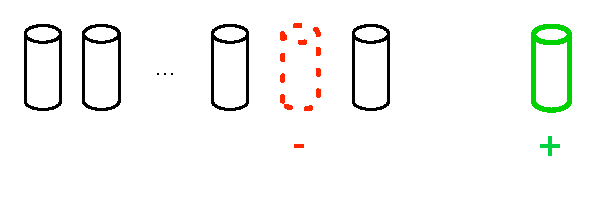
\includegraphics[width=\textwidth]{fig/exchange-multi}
	\caption{An member of $\B_{\Matroid(n)}$.}
	\label{fig:exchange:topk}	
\end{subfigure}
~
\begin{subfigure}[c]{0.25\textwidth}
	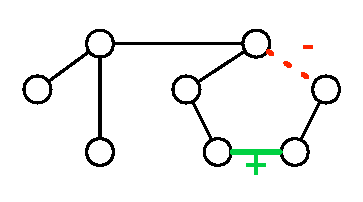
\includegraphics[width=\textwidth]{fig/exchange-matroid}
	\caption{A member of $\B_{\Matroid(n)}$}
	\label{fig:exchange:matroid}
\end{subfigure}
~
\begin{subfigure}[c]{0.22\textwidth}
	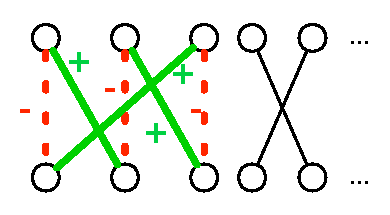
\includegraphics[width=\textwidth]{fig/exchange-match}
	\caption{A member of $\B_{\Match(G)}$.}
\end{subfigure}
~
\begin{subfigure}[c]{0.22\textwidth}
	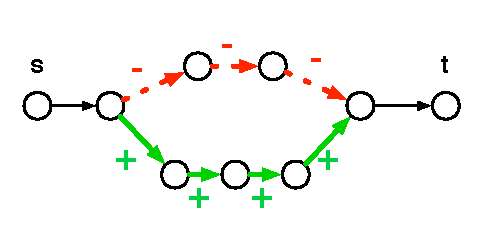
\includegraphics[width=\textwidth]{fig/exchange-path}
	\caption{A member of $\B_{\Path(G,s,t)}$.}
\end{subfigure}
\caption{
Examples of exchange sets belonging to the exchange classes $\B_{\MultiIdent}$, $\B_{\Matroid}$, $\B_{\Match}$ and $\B_{\Path}$:
green-solid elements constitute the set $b_+$, red-dotted elements constitute the set $b_-$ and the example exchange set is $b=(b_+,b_-)$. 
In \Cref{fig:exchange:topk}, we use \MultiIdent as a specific instance of \Matroid.
In \Cref{fig:exchange:matroid}, we use spanning tree as a specific instance of \Matroid.
}
\label{fig:exchange}
\end{figure}
}

 %is also covered by \Cref{example:matroid} (cf. \citep{oxley2006matroid}).
%On the other hand  and \Path cannot be formulated as matroids and in fact these problems are equivalent to matroid intersections (cf. \citep{oxley2006matroid}).

%Many combinatorial problem $\M$ is associated with an exchange class with small width.


%From the definition, it is easy to see that if $\B$ is an exchange class, then, for any $M\not= M'$, there exists a sequence of exchange sets $b_1,\ldots, b_k$ belonging to $\B$ such that $M'=M\oplus b_1 \ldots \oplus b_k$.
%Hence, intuitively, an exchange class for $\M$ characterizes the ``operations'' of transforming an element $M\in \M$ to another element $M'\in \M$.



\section{Lower Bound}
In this section, we present a problem-dependent lower bound on the sample complexity of the \Problem problem. 
To state our results, we first define the notion of \emph{$\delta$-correct algorithm} as follows.
For any $\delta \in (0,1)$, we call an algorithm $\mathbb A$ a $\delta$-correct algorithm if, for any expected reward $\vec w \in \RR^{n}$, the probability of error of $\mathbb A$ is at most $\delta$, i.e. $\Pr[M_*\not =\out] \le \delta$, where $\out$ is the output of algorithm $\mathbb A$.

We show that, for any decision class $\M$ and any expected rewards $\vec w$, any $\delta$-correct algorithm $\mathbb A$ must use at least $\Omega\big(\mathbf H \log(1/\delta) \big)$ samples in expectation.
\begin{restatable}{theorem}{lowerbound}
Fix any decision class $\M\subseteq 2^{[n]}$ and any vector $\vec w \in \RR^n$.
Suppose that, for each arm $e\in [n]$, the reward distribution $\Rew_e$ is given by $\Rew_e=\mathcal N(w(e),1)$, where $\mathcal N(\mu, \sigma^2)$ denotes a Gaussian distribution with mean $\mu$ and variance $\sigma^2$. 
Then, for any $\delta \in (0,e^{-16}/4)$ and any $\delta$-correct algorithm $\mathbb A$, we have
\begin{equation}
\label{eq:lower-bound}
\E[T] \ge \frac{1}{16} \mathbf H \log\left(\frac{1}{4\delta}\right),
\end{equation}
where 
$T$ denote the number of total samples used by algorithm $\mathbb A$ and
$\mathbf H$ is defined in Eq.~\eqref{eq:hardness}.
\label{theorem:lower-bound}
\end{restatable}

%Now we compare the sample complexity Eq.~\eqref{eq:sample-complexity} of \Algorithm to the lower bound provided in Theorem~\ref{theorem:lower-bound} on our running examples \MultiIdent, \Matroid, \Match and \Path.
%For clarity, we consider the case that $\epsilon=0$ which corresponds to the learning problem of finding the optimal set.
%We see that \Algorithm algorithm uses at most $\tilde O(\rank(\B)^2 \mathbf H)$ samples.
%Recall that, for \MultiIdent and \Matroid, Lemma~\ref{lemma:example-exchange-class} shows that $\rank(\B)=2$.
Theorem~\ref{theorem:lower-bound} resolves  the open conjectures of \citet{kalyanakrishnan2012pac} and \citet{bubeck2013multiple} that the lower bounds of sample complexity of \MultiIdent and \MultiBandit problem are $\Omega\big(\mathbf H\log(1/\delta)\big)$.
In addition, in \Cref{example:topk} and \Cref{example:matroid}, we have shown that the sample complexity of \Algorithm is $O(\mathbf H\log(n\mathbf H/\delta))$ for \MultiIdent, \MultiBandit and more generally the decision classes derived from matroids $\M_{\Matroid(T)}$.
Hence, we see that the \Algorithm algorithm achieves the optimal sample complexity within logarithmic factors for these pure exploration problems.

%On the other hand, for $\Match(V,E)$ and $\Path(V,E)$, we see that the gap between the upper bound Eq.~\eqref{eq:sample-complexity} and this lower bound is a factor of $|V|^2$.
On the other hand, for general decision classes with non-constant widths, we see that there is a gap of $\tilde \Theta(\rank(\M)^2)$ between the upper bound Eq.~\eqref{eq:sample-complexity} and the lower bound Eq.~\eqref{eq:lower-bound}.
Notice that we have $\rank(\M) \le n$ for any decision class $\M$ and therefore the gap is relatively benign.
%Ignoring the logarithmic factors, this gap only depends on the underlying combinatorial structure of $\M$.
Our lower bound also suggests that the dependency on $\mathbf H$ of the sample complexity of \Algorithm cannot be improved up to logarithmic factors.
Furthermore, we conjecture that the sample complexity lower bound might inherently depend on the size of exchange sets. 
In the supplementary material, we provide evidence on this conjecture which is a lower bound on the sample complexity of exploration of exchange sets.
 %dependency on $\rank(\M)$ of the sample complexity might be intrinsic. 
%In the supplementary material, we provide evidence showing that the sample complexity of any $\delta$-correct algorithm should be related to size of exchange sets. 


\section{Fixed Budget Algorithm}
In this section, we present \AlgorithmBud, a parameter-free learning algorithm for the \Problem problem in the fixed budget setting.
We analyze the probability of error \AlgorithmBud using the tools of exchange classes.
Recall that, in the fixed budget setting, an algorithm is given a budget $T>0$ such that the algorithm can use at most $T$ pulls.
The goal of the algorithm is to minimize the probability of error. 

\textbf{Constrained oracle.} 
The \AlgorithmBud algorithm requires access to a \emph{constrained oracle}, which is a function denoted as $\COracle: \RR^{n}\times 2^{[n]} \times 2^{[n]} \rightarrow \M$.
The function $\COracle$ takes three inputs: (1) a weight vector $\vec v$, (2) a set $A$ of positive constraints and (3) a set $B$ of negative constraints and returns a solution such that
\begin{equation}
\COracle(\vec v, A, B) \in \argmax_{M: M\in \M, A\subseteq M, B\cap M =\emptyset} v(M).
\end{equation}
Hence we see that $\COracle(\vec v, A, B)$ computes an optimal solution that includes all elements of $A$ while excluding all elements of $B$.
%It is clear that constrained oracles exist for many combinatorial problems including the four examples we considered in this paper.
In the supplementary material, we show that constrained oracles can be easily reduced to maximization oracles by modifying the weight vector according to the constraints. 
In addition, similar to \Algorithm, \AlgorithmBud does not need any additional knowledge of $\M$ other than accesses to a constrained oracle for $\M$.


\textbf{Algorithm.}
The idea of the \AlgorithmBud algorithm is as follows.
The \AlgorithmBud algorithm divides the budget of $T$ rounds into $n$ phases. 
In the end of each phase, \AlgorithmBud either accepts or rejects a single arm. 
If an arm is accepted, then it is included into the final output. 
Conversely, if an arm is rejected, then it is excluded from the final output.
The arms that are neither accepted nor rejected are sampled for a equal number of times in the next phase.
\junk{We see that the major challenge here is to choose a correct arm to accept/reject. 
For decision classes with non-trivial combinatorial structures, one cannot simply accept/reject arms according to their empirical means, since an arm with small expected reward may belong to the optimal set.
We resolve this challenge by using a novel gap estimation method for decision making and demonstrate that \AlgorithmBud can achieve a small probability of error.}

Now we describe the procedure of the \AlgorithmBud algorithm for choosing an arm to accept/reject.
Let $A_t$ denote the set of accepted arms before phase $t$ and let $B_t$ denote the set of rejected arms before phase $t$.
We call an arm $e$ to be active if $e\not\in A_t\cup B_t$.
Then, in phase $t$, \AlgorithmBud samples each active arm for $\tilde T_t -\tilde T_{t-1}$ times, where the definition of $\tilde T_t$ is given in Algorithm~\ref{algo:budget}.
Next, \AlgorithmBud calls the constrained oracle to compute an optimal solution $M_t$ with respect to the empirical means $\bar w_t$, accepted arms $A_t$ and rejected arms $B_t$, i.e. let $M_t = \COracle(\vec {\bar w}_t, A_t,B_t)$.
Then, for each arm active arm $e$, \AlgorithmBud estimate the gap of $e$ in the following way.
If $e\in M_t$, then \AlgorithmBud computes an optimal solution $\tilde M_{t,e}$ that does not include $e$, i.e. $\tilde M_{t,e} = \COracle(\vec {\bar w}_t, A_t, B_t \cup \{e\})$.
Conversely, if $e\not\in M_t$, then \AlgorithmBud computes an optimal $\tilde M_{t,e}$ which includes $e$, i.e. $\tilde M_{t,e} = \COracle(\vec {\bar w}_t, A_t \cup \{e\}, B_t)$.
Then, the gap of $e$ is calculated as $\bar w_t(M_t)-\bar w_t(\tilde M_{t,e})$.
Finally, \AlgorithmBud chooses the  arm $p_t$ with the largest gap.
If $p_t\in M_t$ then $p_t$ is accepted otherwise $p_t$ is rejected.
The pseudo-code of \AlgorithmBud is shown in Algorithm~\ref{algo:budget}.

\begin{algorithm}[htbp]
{
\small
\begin{algorithmic}[1]
\Require Budget: $T>0$; Constrained oracle: $\COracle: \RR^n\times 2^{[n]} \times 2^{[n]} \rightarrow \M$.
\State Define $\barlog(n) \triangleq \sum_{i=1}^n \frac1i$
\State $\tilde T_0 \gets 0, A_1 \gets \emptyset, B_1\gets \emptyset$
\For{$t=1,\ldots,n$}
	\State $\tilde T_t \gets \left\lceil \frac{T-n}{\barlog(n)(n-t+1)} \right\rceil$
	\State Pull each arm $e\in [n]\del (A_t\cup B_t)$ for $\tilde T_t - \tilde T_{t-1}$ times
	\State Update the empirical means $\vec {\bar w}_t\in \RR^n$ of each arm
	\State $M_t \gets \COracle(\vec {\bar w}_t, A_t, B_t)$
	\For{\textbf{each} $e \in [n]\del (A_t\cup B_t)$}
		\If {$e\in M_t$}
			\State $\tilde M_{t,e} \gets \COracle(\vec {\bar w}_t, A_t, B_t \cup \{e\})$
	  \Else
	    \State $\tilde M_{t,e} \gets \COracle(\vec {\bar w}_t, A_t \cup \{e\}, B_t)$
	  \EndIf
	\EndFor
	\State $p_t \gets \argmax_{i\in[n]\del (A_t\cup B_t)} \bar w_t(M_t) - \bar w_t(\tilde M_{t,i})$
	\If {$p_t\in M_t$}
		\State $A_{t+1} \gets A_t \cup \{p_t\}, B_{t+1} \gets B_t$
	\Else
		\State $A_{t+1} \gets A_t , B_{t+1} \gets B_t \cup \{p_t\}$
	\EndIf
\EndFor
\State $\out\gets A_{n+1}$
\State \textbf{return} $\out$
\end{algorithmic}
}
\caption{\AlgorithmBud: Combinatorial Gap-based Elimination}
\label{algo:budget}
\end{algorithm}


\subsection{Analysis}
In the following theorem, we show that the probability of error of the \AlgorithmBud algorithm is at most $\tilde O(\exp(-T\rank(\M)^{-2} \mathbf H^{-1}))$.
\begin{restatable}{theorem}{realfixbudget}
Use the same notations as in Theorem~\ref{theorem:main}.
Let $\Delta_{(1)},\ldots,\Delta_{(n)}$ be a permutation of $\Delta_1,\ldots,\Delta_n$ such that
$\Delta_{(1)} \le \ldots \ldots \Delta_{(n)}$. 
Define $\mathbf H_2 \triangleq \max_{i\in[n]} i\Delta_{(i)}^{-2}$.
Then, given any budget $T > n$, the \AlgorithmBud algorithm uses at most $T$ samples and outputs a solution $\out \in \M$ such that
\begin{equation}
\Pr[\out\not=M_*] \le n^2  \exp\left(-\frac{2(T-n)}{9R^2 \barlog(n) \rank(\M)^2 \mathbf H_2} \right),
\label{eq:fbudget:prob-error}
\end{equation}
where $\barlog(n)\triangleq \sum_{i=1}^n \frac1i$.
\label{theorem:budget}
\end{restatable}
The quantity $\mathbf H_2$ defined in Theorem~\ref{theorem:budget} can be considered as a surrogate of $\mathbf H$ since these two quantities are equivalent up to a logarithmic factor: $\mathbf H_2 \le \mathbf H \le \log(2n) \mathbf H_2$.
Applying Theorem~\ref{theorem:budget} to the \MultiIdent problem, we see that our bound matches previous fixed budget algorithm due to \citet{bubeck2013multiple}.

We see that $\rank(\M)^2$ also appears in the probability of error Eq.~\eqref{eq:fbudget:prob-error} in Theorem~\ref{theorem:budget}, which indicates that $\rank(\M)$ may reflect the inherent hardness associate with a decision class $\M$ for the \Problem problem.
%Moreover, the analysis of \AlgorithmBud re-uses many tools and ideas within the framework of exchange classes which are developed for the analysis of our main algorithm \Algorithm.
%We use these tools to design gadgets in order to bound the estimations of gaps.
%This suggests that the framework of exchange class may be of interest for the analysis of other similar on-line combinatorial optimization problems.
We also notice that the \AlgorithmBud algorithm uses solely the empirical means of arms to support its decision making; while our main algorithm \Algorithm uses explicitly constructed confidence intervals of the arms.
From this viewpoint, the \AlgorithmBud algorithm is quite different from our main algorithm \Algorithm. 
This actually leads to an argument substantially different from the proof of Theorem~\ref{theorem:main}. 
%And we have to build different gadgets using the exchange classes.

\section{Related Work}

The multi-armed bandit problem has been extensively studied in both stochastic and adversarial settings \citep{lai1985asymptotically,auer2002nonstochastic,auer2002nonstochastic}.
We refer readers to \citep{bubeck2012regret} for a survey on recent results.
Many work on MABs focus on minimizing the cumulative regret, which is an objective known to be fundamentally different from the objective of pure exploration MABs \citep{bubeck2010pure}.
Among these work, a recent line of research considers a generalized setting called combinatorial bandits in which a set of arms (satisfying certain combinatorial constraint) is played on each round \citep{cesa2012combinatorial,chen2013combinatorial,kale2010non,neu2010online,audibert2009minimax,Bubeck12towardsminimax}.
Note that the objective of these work is to minimize the cumulative regret, which differs from ours.

In the literature of pure exploration MABs, the classical problem of identifying the single best arm has been well-studied in both fixed confidence and fixed budget settings \citep{mannor2004sample,bubeck2010pure,audibert2010best,gabillon2012best,jamieson2013lil,jamieson2014best}.
A flurry of recent work extend this classical problem to \MultiIdent and \MultiBandit problems and provide algorithms and upper bounds \citep{kalyanakrishnan2010efficient,kalyanakrishnan2012pac,zhou2014optimal,bubeck2013multiple,NIPS2011_4478,gabillon2012best}.
Our framework encompasses these two problems as special cases and covers a much larger class of structured pure exploration problems, which are unaddressed in the current literature.
Applying our results back to \MultiIdent and \MultiBandit, our upper bounds match the best known problem-dependent bounds due to \citet{gabillon2012best} and \citet{bubeck2013multiple}; and our lower bound provides the first problem-dependent lower bounds for these two problems, which are conjectured earlier by \citet{kalyanakrishnan2012pac} and \citet{bubeck2013multiple}.
%We also notice that a very recent due to XXX improves 
%In addition, to our knowledge, there is no known problem-dependent lower bounds for \MultiIdent and \MultiBandit. 
%Therefore, when applying our general lower bound to \MultiIdent and \MultiBandit, we obtain the first problem-dependent lower bounds for these two problems. 
%Our result also shows that our upper bound is essentially tight (up to logarithmic factors) for these two problems.

\section{Conclusion}
In this paper, we proposed a general framework called \Problem which represents a rich class of structured pure exploration problems and admits potential applications in various domains.
We have shown a number of results for the framework, including two novel learning algorithms, their related upper bounds and a novel lower bound.
The proposed algorithms support a wide range of decision classes in a unifying way and our analysis introduced a novel tool called exchange class which maybe of independent interest.
Our upper and lower bounds characterize the complexity of the \Problem problem: the sample complexity of our algorithm is optimal (up to a logarithmic factor) for the decision classes derived from matroids (including \MultiIdent and \MultiBandit), while for general decision classes, our upper and lower bounds are within a relatively benign factor.
%We presented two learning algorithms  for the \Problem problem in both fixed confidence (\Algorithm) and fixed budget settings (\AlgorithmBud) and proved problem-dependent performance guarantees using a novel tool called exchange class.
%The proposed algorithms support a wide range of decision classes and only require accesses to a maximization oracle.
%We also established a general sample complexity lower bound for the \Problem problem, which shows that the sample complexity of our algorithm is optimal (up to a logarithmic factor) for the decision classes derived from matroids (including \MultiIdent and \MultiBandit), while for general decision classes, our upper and lower bound are within a relatively benign factor.
%Furthermore, we extended \Algorithm to fixed budget setting and PAC learning setting.
%Our results substantially improve upon the existing work on pure exploration MABs of identifying sets of arms. 
%Our improvements are diverse, which range form considering a much larger 




%We claim that $e\in (M_{t,e}' \cap \neg M_t) \cup (\neg M_{t,e}' \cap M_t)$.
%Therefore it is easy to see that $$

\newpage
\bibliography{bandit}
\bibliographystyle{my-plainnat}

\newpage
\appendix

\maketitle


\section{Proof of Main Result}

In this section, we prove our main result: Theorem~\ref{theorem:main}.


\textbf{Notations.} 
We need some additional notations for our analysis.
For any set $a\subseteq [n]$, let $\vec \chi_a \in \{0,1\}^n$ denote the incidence vector of set $a \subseteq [n]$, i.e. $\chi_a(e) = 1$ if and only if $e\in a$.
For an exchange set $b=(b_+,b_-)$, we define $\vec \chi_b \triangleq \vec \chi_{b_+}- \vec \chi_{b_-}$ as the incidence vector of $b$.
We notice that $\vec \chi_b \in \{-1,0,1\}^n$.

For each round $t$, we define vector $\vec\rad_t = \big(\rad_t(1),\ldots,\rad_t(n)\big)^T$ and recall that $\vec {\bar w}_t\in \RR^n$ is the empirical mean rewards of arms up to round $t$.

Let $\vec u\in \RR^n$ and $\vec v\in \RR^n$ be two vectors.
Let $\inn{\vec u, \vec v}$ denote the inner product of $\vec u$ and $\vec v$.
We define $\vec u \odot \vec v \triangleq \big(u(1)\cdot v(1),\ldots,u(n)\cdot v(n)\big)^T$ as the element-wise product of $\vec u$ and $\vec v$.
For any $s\in \RR$, we also define $\vec u^s \triangleq \big(u(1)^s, \ldots, u(n)^s)^T$ as the element-wise exponentiation of $\vec u$.
Let $|\vec u| = \big(|u(1)|, \ldots, |u(n)|\big)^T$ denote the element-wise absolute value of $\vec u$.



\subsection{Preparatory Lemmas}
%We define $w_t(a) = \langle \vec {\bar w}_t, \vec \chi_a \rangle$ and $\rad_t(a) = \langle \vec\rad_t, \left|\vec \chi_a \right| \rangle$, where $a$ is a set or an exchange set and $\vec \chi_a$ is the incidence vector of $a$. 


\begin{lemma}
Let $M_1 \subseteq [n]$ be a set.
Let $b=(b_+,b_-)$ be an exchange set such that 
$b_-\subseteq M_1$ and $b_+ \cap M_1 = \emptyset$.
Define $M_2 = M_1 \oplus b$.
Then, we have 
$$
\vec\chi_{M_1} +\vec\chi_{b} = \vec\chi_{M_2}.
$$
\label{lemma:exchange-char}
\end{lemma}

\begin{proof}
Recall that $M_2 = M_1 \del b_- \oplus b_+$ and $b_+\cap b_-=\emptyset$.
Therefore we see that $M_2 \del M_1 = b_+$ and $M_1 \del M_2 = b_-$.
Then, we decompose $\vec\chi_{M_1}$ as $\vec\chi_{M_1}=\vec\chi_{M_1\del M_2}+\vec\chi_{M_1\cap M_2}$.
Hence, we have
\begin{align*}
   \vec\chi_{M_1}+\vec\chi_{b} &= \vec\chi_{M_1\del M_2}+\vec\chi_{M_1\cap M_2} + \vec\chi_{b_+}-\vec\chi_{b_-}\\
   							   &= \vec\chi_{M_1\cap M_2} + \vec\chi_{M_2\del M_1}\\
   							   &= \vec\chi_{M_2}.
\end{align*}
\end{proof}


\begin{lemma}
\label{lemma:exchange}
Let $\M\subseteq 2^{[n]}$ and $\B$ be an exchange class for $\M$.
Then, for any two different elements $M,M'$ of $\M$ and any $e \in (M\del M')\cup(M'\del M)$, there exists an exchange set $b=(b_+,b_-) \in \B$ such that
$e\in (b_+\cup b_-)$, $b_-\subseteq (M\del M')$, $b_+\subseteq (M'\del M)$, 
$(M\oplus b) \in \M$ and  $(M'\ominus b) \in \M$.
%In addition, the incidence vectors are related by $\vec \chi_M +\vec \chi_b = \vec \chi_{M \oplus b}$.
Moreover, if $M' = M_*$, then we have $\inn{\vec w, \vec \chi_b} \ge \Delta_e > 0$,
where $\Delta_e$ is the gap defined in Eq.~\eqref{eq:define-delta}.
\end{lemma}

\begin{proof}
We decompose our proof into two cases.

\textbf{Case (1): $e\in M\del M'$.}

By the definition of exchange class, we know that 
there exists $b=(b_+, b_-) \in \B$ which satisfies that
$e\in b_-$, $b_- \subseteq (M\del M') $, $b_+\subseteq (M' \del M)$, $(M\oplus b) \in \M$ and $(M'\ominus b) \in \M$.

Next, if $M'=M_*$, we see that $e\not \in M_*$.
Let us consider the set $M_1 = \argmax_{M': M'\in \M \wedge e\in M'} w(M')$.
Also define $M_0 = M_*\ominus b$. 
We have already proved that $M_0\in \M$.  
%Since $e\in M_1$, we see that $M_1\not= M_*$.
Combining with the fact that $e\in M_0$, we see that $w(M_0) \le w(M_1)$. 
Therefore, we obtain that
$w(M_*)-w(M_0) \ge w(M_*)-w(M_1) = \Delta_e$.
Notice that the left-hand side of the former inequality can be rewritten using Lemma~\ref{lemma:exchange-char} as follows
$$
w(M_*)-w(M_0) = \inn{\vec w, \vec \chi_{M_*}}-\inn{\vec w, \vec \chi_{M_0}} = \inn{\vec w, \vec \chi_{M_*}-\vec\chi_{M_0}}
= \inn{\vec w,\vec \chi_b}.
$$
Therefore, we obtain $\inn{\vec w,\vec \chi_b} \ge \Delta_e$.
%We decompose $\vec \chi_M = \vec \chi_{M\del M'}+\vec\chi_{M \cap M'}$.
%Recall that $\vec \chi_b = \vec \chi_{b_+}-\vec\chi_{b_-}$

\textbf{Case (2): $e\in M'\del M$.}

Using the definition of exchange class, we see that 
there exists $c=(c_+,c_-)\in \B$ such that 
$e\in c_-$, $c_-\subseteq (M'\del M)$, $c_+\subseteq (M\del M')$, $(M'\oplus c)\in \M$
and $(M\ominus c)\in \M$.

We construct $b=(b_+,b_-)$ by setting $b_+=c_-$ and $b_-=c_+$. 
Notice that, by the construction of $b$, we have $M\oplus b = M\ominus c$ and $M'\ominus b = M'\oplus c$.
Therefore, it is clear that $b$ satisfies the requirement of the lemma.


Now, suppose that $M'=M_*$. 
In this case, we have $e\in M_*$.
Consider the set $M_3 = \argmax_{M': M'\in \M \wedge e\not \in M'} w(M')$.
We see that $w(M_*)-w(M_3)=\Delta_e$.
Define $M_2 = M_* \ominus b$ and notice that  $M_2 \in \M$.
Combining with the fact that $e\not \in M_2$, we obtain that $w(M_2) \le w(M_3)$.
Hence, we have
$w(M_*)-w(M_2) \ge w(M_*)-w(M_3)=\Delta_e$.
Similar to Case (1), applying Lemma~\ref{lemma:exchange-char} again, we have
$$
\inn{\vec w,\vec \chi_b} = w(M_*)-w(M_2) \ge \Delta_e.
$$


\end{proof}

\begin{lemma}
\label{lemma:max}
Let $M$ and $M'$ be two sets. 
Then, we have 
$$ \max_{e \in (M\del M') \cup (M'\del M)} \rad_t(e) = \big\|\vec \rad_t \odot |\vec \chi_{M'} - \vec \chi_M| \big\|_\infty.$$
\end{lemma}

\begin{proof}
Notice that $\vec\chi_{M'}-\vec\chi_{M} = \vec\chi_{M'\del M}-\vec\chi_{M\del M'}$.
In addition, since $(M'\del M) \cap (M\del M') = \emptyset$, we have
$\vec \chi_{M'\del M} \odot \vec\chi_{M\del M'} = \vec 0_n$. 
Also notice that $ \vec\chi_{M'\del M}-\vec\chi_{M\del M'} \in \{-1,0,1\}^n$.
Therefore, we have
\begin{align*}
|\vec\chi_{M'\del M}-\vec\chi_{M\del M'}| 
&= (\vec\chi_{M'\del M}-\vec\chi_{M\del M'})^2\\
&=\vec\chi_{M'\del M}^2+\vec\chi_{M\del M'}^2+2\vec \chi_{M'\del M} \odot \vec\chi_{M\del M'} \\
&=\vec\chi_{M'\del M}+\vec\chi_{M\del M'}\\
& = \vec\chi_{(M' \del M) \cup (M\del M')},
\end{align*}
where the third equation follows from the fact that $\vec\chi_{M\del M'}\in \{0,1\}^n$ and $\vec\chi_{M'\del M}\in\{0,1\}^n$.
The lemma follows immediately from the fact that $\rad_t(e) \ge 0$ and  $\vec\chi_{(M\del M')\cup(M'\del M)}\in \{0,1\}^n$.
\end{proof}

\begin{lemma}
\label{lemma:vector-technical}
Let $\vec a,\vec b, \vec c \in \RR^n$ be three vectors.
Then, we have $\inn{\vec a, \vec b\odot \vec c} = \inn{\vec a\odot \vec b,\vec c}$.
\end{lemma}

\begin{proof}
We have
\begin{align*}
	\inn{\vec a,\vec b\odot \vec c} = \sum_{i=1}^n a(i) \big(b(i) c(i)\big) = \sum_{i=1}^n \big(a(i)b(i)\big)c(i) = \inn{\vec a\odot\vec b,\vec c}.
\end{align*}
\end{proof}

\begin{lemma}
Let $M_t$ and $\vec{\tilde w_t}$ be defined in Algorithm~1. 
Let $M' \in \M$ be a feasible set.
We have
$$
\tilde w_t(M')-\tilde w_t(M_t) = 
\inn{\vec{\tilde w}_t, \vec \chi_{M'}-\vec \chi_{M_t}} = \inn{\vec {\bar w}_t, \vec \chi_{M'}-\vec\chi_{M_t}}+\inn{\vec \rad_t, |\vec \chi_{M'}-\vec\chi_{M_t}|}.
$$
\label{lemma:tilde}
\end{lemma}

\begin{proof}
We begin with proving the first part.
It is easy to verify that $\vec {\tilde w_t} = \vec {\bar w}_t+ \vec \rad_t \odot (\vec 1_n-2\vec\chi_{M_t})$.
Then, we have
\begin{align}
\inn{\vec{\tilde w}_t, \vec \chi_{M'}-\vec \chi_{M_t}}
&= \inn{\vec {\bar w}_t+ \vec \rad_t \odot (1-2\vec\chi_{M_t}), \;\vec \chi_{M'}-\vec \chi_{M_t}} \nonumber \\
&= \inn{\vec {\bar w}_t,\vec \chi_{M'}-\vec \chi_{M_t}}+\inn{\vec \rad_t, (\vec 1_n-2\vec\chi_{M_t}) \odot (\vec \chi_{M'}-\vec \chi_{M_t})}
\label{eq:l-d-1}\\
&= \inn{\vec {\bar w}_t,\vec \chi_{M'}-\vec \chi_{M_t}}+\inn{\vec \rad_t, \vec\chi_{M'}-\vec\chi_{M_t}-2\vec\chi_{M_t}\odot\vec\chi_{M'}+2\vec\chi_{M_t}^2 } \nonumber\\
&= \inn{\vec {\bar w}_t,\vec \chi_{M'}-\vec \chi_{M_t}}+\inn{\vec \rad_t, \vec\chi_{M'}^2-\vec\chi_{M_t}^2-2\vec\chi_{M_t}\odot\vec\chi_{M'}+2\vec\chi_{M_t}^2 }
\label{eq:l-d-2}\\
&= \inn{\vec {\bar w}_t,\vec \chi_{M'}-\vec \chi_{M_t}}+\inn{\vec \rad_t, (\vec\chi_{M'}-\vec\chi_{M_t})^2}
\nonumber \\ \
&= \inn{\vec {\bar w}_t,\vec \chi_{M'}-\vec \chi_{M_t}}+\inn{\vec \rad_t, \big|\vec\chi_{M'}-\vec\chi_{M_t}\big|},
\label{eq:l-d-3}
\end{align}
where
Eq.~\eqref{eq:l-d-1} follows from Lemma~\ref{lemma:vector-technical};
Eq.~\eqref{eq:l-d-2} holds since $\vec \chi_{M'}\in \{0,1\}^n$ and $\vec \chi_{M_t}\in \{0,1\}^n$
and therefore $\vec\chi_{M'}=\vec\chi_{M'}^2$ and $\vec\chi_{M_t}=\vec\chi_{M_t}^2$;
and Eq.~\eqref{eq:l-d-3} follows since $\vec\chi_{M'}-\vec\chi_{M_t}\in \{-1,0,1\}^n$.
\junk{
Next, recall that $\tilde M_t = \argmax_{M\in \M} \tilde w_t(M)$.
Therefore, we have $\tilde w_t(\tilde M_t) \ge \tilde w_t(M')$.
Subtracting $\tilde w_t(M_t)$ from both sides of the former inequality, we have
\begin{equation}
\tilde w_t(\tilde M_t)-\tilde w_t(M_t) \ge \tilde w_t(M')-\tilde w_t(M_t).
\label{eq:l-d-4}
\end{equation}
The lemma follows by noticing that the left-hand side of Eq.~\eqref{eq:l-d-4} equals to 
$\inn{\vec {\bar w}_t,\vec \chi_{\tilde M_t}-\vec \chi_{M_t}}+\inn{\vec \rad_t, \big|\vec\chi_{\tilde M_t}-\vec\chi_{M_t}\big|}$
and the right-hand side equals to
$\inn{\vec {\bar w}_t,\vec \chi_{M'}-\vec \chi_{M_t}}+\inn{\vec \rad_t, \big|\vec\chi_{M'}-\vec\chi_{M_t}\big|}$.
}
\end{proof}


\subsection{Confidence Intervals}

For all $t>0$, we define random event $\xi_t$ as follows
\begin{equation}
\xi_t = \Big\{
\forall i\in[n],\quad 
|w(i)-\bar w_t(i)| \le \rad_t(i) 
\Big\}.
\label{eq:define-xi}
\end{equation}
We notice that random event $\xi_t$ characterizes the event that the confidence bounds of all arms are valid at round $t$.

If the confidence bounds are valid, we can generalize Eq.~\eqref{eq:define-xi} to inner products as follows.
\begin{lemma}
\label{lemma:ci-property}
Given any $t>0$, assume that event $\xi_t$ as defined in Eq.~\eqref{eq:define-xi} occurs. 
Then, for any vector $\vec a \in \RR^n$, we have
$$
\big|\inn{\vec w,\vec a} - \inn{\vec {\bar w}_t, \vec a}\big| \le \inn{\vec \rad_t, |\vec a|}.
$$
\end{lemma}

\begin{proof}
Suppose that $\xi_t$ occurs. Then, we have
\begin{align}
\big|\inn{\vec w,\vec a} - \inn{\vec {\bar w}_t, \vec a}\big| 
&=\big|\inn{\vec w-\vec {\bar w}_t,\vec a}\big| \nonumber \\
&=\left|\sum_{i=1}^n \big(w(i)-\bar w_t(i)\big) a(i)  \right| \nonumber \\
&\le\sum_{i=1}^n \big| w(i)-\bar w_t(i)\big| |a(i)| \nonumber \\
&\le\sum_{i=1}^{n} \rad_t(i) \cdot |a(i)| \label{eq:ci-c-1}\\
&= \inn{\vec \rad_t,  |\vec a|}, \nonumber
\end{align}
where Eq.~\eqref{eq:ci-c-1} follows the definition of event $\xi_t$ in Eq.~\eqref{eq:define-xi} and the assumption that it occurs.
\end{proof}


Next, we construct the high probability confidence intervals for the fixed confidence setting.
\begin{lemma}
\label{lemma:ci}
Suppose that the reward distribution $\Rew_e$ is a $R$-sub-Gaussian distribution for all $e\in [n]$.
And if, for all $t>0$ and all $e\in [n]$, 
the confidence radius $\rad_t(e)$ is given by
$$
\rad_t(e) = R\sqrt{\frac{2\log\left(\frac{4n t^2}\delta\right)}{T_e(t)}},
$$
where $T_e(t)$ is the number of samples of arm $e$ up to round $t$.
Then, we have
$$
\Pr\left[\bigcap_{t=1}^\infty \xi_t \right] \ge 1-\delta.
$$
\end{lemma}

\begin{proof}
%We claim that, for any $t>0$, one has $\Pr[\xi_t] \ge 1- \frac{\delta}{4t^2}$.
For any $t>0$ and $e\in [n]$, notice $\Rew_e$ is a $R$-sub-Gaussian distribution with mean $w(e)$ and $w_t(e)$ is the empirical mean of $\Rew_e$ for $T_e(t)$ samples. 
Using Hoeffding's inequality (see Lemma~\ref{lemma:hoeffeding} in Section~\ref{section:technical}), we obtain
$$
\Pr\left[ \big|\bar w_t(e)-w(e) \big| \ge R\sqrt{\frac{2\log\left(\frac{4n t^2}\delta\right)}{T_e(t)}} \right] \le \frac{\delta}{2nt^2}.
$$
By union bound over all $e\in [n]$, we see that $\Pr[\xi_t] \ge 1-\frac{\delta}{2t^2}$. 
Using a union bound again over all $t>0$, we have
\begin{align*}
\Pr\left[\bigcap_{t=1}^\infty \xi_t \right] &\ge 1-\sum_{t=1}^\infty \Pr[\neg \xi_t]\\
&\ge 1-\sum_{t=1}^\infty \frac{\delta}{2t^2}\\
&= 1-\frac{\pi^2}{12}\delta \ge 1-\delta.
\end{align*}
\end{proof}



\subsection{Main Lemmas}

\begin{lemma}
\label{lemma:correct}
Given any $t > 0$, assume that event $\xi_t$ (defined in Eq.~\eqref{eq:define-xi}) occurs.
Then, if Algorithm~\ref{algo:pac} terminates at round $t$, we have $M_t=M_*$.
\end{lemma}

\begin{proof}
Suppose that $M_t \not= M_*$. 
By definition, we have $w(M_*)>w(M_t)$. 
Rewriting the former inequality, we obtain that $\inn{\vec w, \vec\chi_{M_*}} > \inn{\vec w,\vec\chi_{M_t}}$.

Applying Lemma~\ref{lemma:exchange} by setting $M=M_t$ and $M'=M_*$, we see that 
there exists $b=(b_+,b_-)\in \B$ such that $(M_t \oplus b) \in \M$.
%Then, using Lemma~\ref{lemma:exchange-char}, we see that 


Now define $M_t' = M_t \oplus b$.
Recall that $\tilde M_t =\argmax_{M\in \M} \tilde w_t(M)$ and therefore $\tilde w_t(\tilde M_t) \ge \tilde w_t(M_t')$.
Hence, we have
\begin{align}
  \tilde w_t(\tilde M_t)-\tilde w_t(M_t) 
  &\ge \tilde w_t(M_t')-\tilde w_t(M_t) \nonumber \\
  &= \inn{\vec {\bar w}_t, \vec \chi_{M_t'}-\vec\chi_{M_t}}+\inn{\vec \rad_t, |\vec \chi_{M'}-\vec\chi_{M_t}|} \label{eq:lc-1}\\
  &\ge \inn{\vec w, \vec \chi_{M_t'}-\vec\chi_{M_t}} \label{eq:lc-2}\\
  &= w(M_t')-w(M_t) > 0 \label{eq:lc-3},
\end{align}
where Eq.~\eqref{eq:lc-1} follows from Lemma~\ref{lemma:tilde};
and Eq.~\eqref{eq:lc-2} follows the assumption that event $\xi_t$ occurs and Lemma~\ref{lemma:ci-property};

Therefore Eq.~\eqref{eq:lc-3} shows that $\tilde w_t(\tilde M_t) > \tilde w_t(M_t)$. 
However, this contradicts to the stopping condition of \Algorithm: $\tilde w_t(\tilde M_t) \le \tilde w_t(M_t)$ and the assumption that the algorithm terminates on round $t$.
\end{proof}




\begin{lemma}
\label{lemma:key-technical}
Given any $t>0$ and suppose that event $\xi_t$ (defined in Eq.~\eqref{eq:define-xi})  occurs.
%Let $\B$ be an exchange class for $\M$.
For any $e\in [n]$, if $\rad_t(e) < \frac{\Delta_e}{3\rank(\M)}$, then, arm $e$ will not be pulled on round $t$, i.e. $p_t\not= e$.
\end{lemma}

\begin{proof}
Fix an exchange class $\B\in \argmin_{\B'\in \Exchange(\M)} \rank(\B')$.
Suppose, in the contrary, that $p_t = e$.
By Lemma~\ref{lemma:exchange}, there exists an exchange set $c=(c_+,c_-) \in \B$
such that $e\in (c_+\cup c_-)$, $c_- \subseteq (M_t \del \tilde M_t)$, $c_+ \subseteq (\tilde M_t \del M_t)$, $(M_t\oplus c) \in \M$ and $(\tilde M_t \ominus c) \in \M$.

%Define vector 

Now, we decompose our proof into two cases.

\textbf{Case (1): $(e \in M_* \wedge e\in c_+) \vee (e \not \in M_* \wedge e\in c_-)$.}

Define $M_t' = \tilde M_t \ominus c$ and recall that $M_t' \in \M$ due to the definition of exchange class.

First, we claim that $M_t'\not= M_*$.
Suppose that $e\in M_*$ and $e\in c_+$.
Then, we see that $e\not\in M_t'$ and hence $M_t'\not=M_*$.
On the other hand, if $e\not \in M_*$ and $e\in c_-$, then $e\in M_t'$ which also means that $M_t'\not= M_*$.
Therefore we have $M_t'\not=M_*$ in either cases.

%There exists an exchange set $b=(b_+,b_-)\in \B$ such that $e\in b_+$, $b_+\subseteq (M_* \del M_t')$, $b_- \subseteq (M_t'\del M_*)$ and $M_t'\oplus b \in \M$.

Next, we apply Lemma~\ref{lemma:exchange} by setting $M=M_t'$ and $M'=M_*$.
We see that there exists an exchange set $b\in \B$ such that, $e\in (b_+\cup b_-)$, $(M_t' \oplus b) \in \M$ and
 $\inn{\vec w, \vec \chi_b} \ge \Delta_e > 0$.
 
Now, we define vectors $\vec d = \vec \chi_{\tilde M_t} - \vec \chi_{M_t}$, $\vec d_1 = \vec\chi_{M_t'}-\vec\chi_{M_t}$ and $\vec d_2 = \vec\chi_{M_t'\oplus b}-\vec\chi_{M_t}$.
%It is clear that $d\in[0,1]^n$,$d_1\in[0,1]^n$ and $d_2\in[0,1]^n$.
By the definition of $M_t'$ and Lemma~\ref{lemma:exchange}, we see that $\vec d_1 = \vec d - \vec \chi_{c}$ and $\vec d_2 = \vec d_1+\vec \chi_b = \vec d-\vec \chi_c+\vec \chi_b$.


Then, we claim that $\nor{\vec \rad_t \odot (\vec d-\vec \chi_c)}_\infty < \frac{\Delta_e}{3\rank(\B)}$.
Since $c_-\subseteq M_t$ and $c_+\cap M_t = \emptyset$, using standard set theoretical manipulations, we can show that $M_t \del \tilde M_t= (M_t \del M_t') \cup c_-$. 
Similarly, one can show that $\tilde M_t \del M_t = (M_t' \del M_t) \cup c_+$. 
This means that $\big((M_t \del M_t') \cup (M_t'\del M_t)\big) \subseteq \big((M_t \del \tilde M_t ) \cup (\tilde M_t \del M_t)\big)$.
Then, applying Lemma~\ref{lemma:max}, we obtain
\begin{align}
   \nor{\vec \rad_t \odot (\vec d-\vec\chi_c)}_\infty 
   &= \nor{\vec \rad_t \odot (\vec \chi_{M_t'} - \vec\chi_{M_t})}_\infty \nonumber\\
   &= \max_{i\in (M_t \del M_t') \cup (M_t'\del M_t) } \rad_t(i) \nonumber \\
   &\le \max_{i\in (M_t \del \tilde M_t ) \cup (\tilde M_t \del M_t)}  \rad_t(i) \nonumber \\
   & = \rad_t(e) < \frac{\Delta_e}{3\rank(\B)} \label{eq:u-c-1-0}.
\end{align}

We claim that $\nor{\vec \rad_t \odot \vec \chi_c}_\infty < \frac{\Delta_e}{3\rank(\B)}$.
Recall that, by the definition of $c$, we have
$c_+\subseteq (\tilde M_t \del M_t)$ and $c_-\subseteq (M_t\del \tilde M_t)$. 
Hence $c_+\cup c_- \subseteq  (\tilde M_t \del M_t)\cup (M_t\del \tilde M_t)$.
Since $\vec \chi_c \in [-1,1]^n$, we see that 
\begin{align}
\nor{\vec \rad_t \odot |\vec \chi_c|}_\infty &= \max_{i\in  c_+\cup c_-} \rad_t(i) \nonumber \\
									    &\le \max_{i\in  (\tilde M_t \del M_t)\cup (M_t\del \tilde M_t)} \rad_t(i)  \nonumber \\
									    &= \rad_t(e) < \frac{\Delta_e}{3\rank(\B)} \label{eq:u-c-1-0-1}.
\end{align}


Next, we claim that $\vec d \odot \vec \chi_c = |\vec \chi_c|$.
Recall that $\vec\chi_c = \vec\chi_{c_+}-\vec\chi_{c_-}$
and $\vec d = \vec \chi_{\tilde M_t}-\vec \chi_{M_t} = \vec\chi_{\tilde M_t\del M_t} - \vec\chi_{M_t\del \tilde M_t}$.
We also notice that $c_+ \subseteq (\tilde M_t \del M_t)$ and $c_- \subseteq (M_t \del \tilde M_t)$.
This implies that $c_+ \cap (M_t \del \tilde M_t) = \emptyset$ and $c_-\cap (\tilde M_t \del M_t) = \emptyset$.
Therefore, we have
\begin{align*}
\vec d \odot \vec \chi_c &= (\vec\chi_{\tilde M_t\del M_t} - \vec\chi_{M_t\del \tilde M_t})\odot(\vec\chi_{c_+}-\vec\chi_{c_-})\\
&= \vec\chi_{\tilde M_t\del M_t}\odot \vec\chi_{c_+}+
   \vec\chi_{M_t \del \tilde M_t}\odot \vec\chi_{c_-}-
   \vec\chi_{\tilde M_t\del M_t}\odot \vec\chi_{c_-}-
   \vec\chi_{M_t\del \tilde M_t}\odot \vec\chi_{c_+}\\
&= \vec\chi_{\tilde M_t\del M_t}\odot \vec\chi_{c_+}+
   \vec\chi_{M_t \del \tilde M_t}\odot \vec\chi_{c_-} \\
&= \vec\chi_{c_+}+\vec\chi_{c_-} =|\vec\chi_c|. 
\end{align*}
where the last equality holds since $c_+\cap c_- =\emptyset$.

Now, we bound  quantity $\langle \vec \rad_t, |\vec d_2| \rangle - \langle \vec \rad_t, |\vec d| \rangle$ as follows
\begin{align}
\langle \vec \rad_t, |\vec d_2| \rangle - \langle \vec \rad_t, |\vec d| \rangle &=
\langle \vec \rad_t, |\vec d_2|-|\vec d| \rangle = \left\langle \vec \rad_t, \vec d_2^2- \vec d^2 \right\rangle
\label{eq:u-c-1-1} \\
&= \left\langle \vec \rad_t, (\vec d-\vec \chi_c+\vec \chi_b)^2- \vec d^2 \right\rangle 
\nonumber \\
&= \left\langle \vec \rad_t, \vec \chi_b^2+\vec \chi_c^2-2\vec \chi_b\odot \vec \chi_c -
						  2\vec d \odot \vec \chi_c + 2\vec d\odot\vec \chi_b \right\rangle
\nonumber \\
&= \left\langle \vec \rad_t, \vec \chi_b^2 - \vec \chi_c^2+2\vec \chi_b\odot (\vec d-\vec \chi_c)\right\rangle
\label{eq:u-c-1-2}\\
&= \left\langle \vec \rad_t, |\vec\chi_b| \right\rangle
  -\left\langle \vec \rad_t, |\vec\chi_c| \right\rangle
  -2\left\langle \vec \rad_t, \vec \chi_b\odot (\vec d-\vec \chi_c) \right\rangle
  \nonumber \\
&= \left\langle \vec \rad_t, |\vec\chi_b| \right\rangle
  -\left\langle \vec \rad_t, |\vec\chi_c| \right\rangle
  -2\left\langle \vec \rad_t \odot (\vec d-\vec \chi_c), \vec \chi_b \right\rangle
  \label{eq:u-c-1-3}\\  
& \ge \left\langle \vec \rad_t, |\vec\chi_b| \right\rangle
  -\left\langle \vec \rad_t, |\vec\chi_c| \right\rangle
  -2\left\|\vec \rad_t \odot (\vec d-\vec \chi_c)\right\|_\infty \left\| \vec \chi_b\right\|_1
  \label{eq:u-c-1-4} \\
& > \left\langle \vec \rad_t, |\vec\chi_b| \right\rangle
  -\left\langle \vec \rad_t, |\vec\chi_c| \right\rangle
  -\frac{2\Delta_e}{3\rank(\B)} \|\vec\chi_b\|_1 
  \label{eq:u-c-1-5}\\
& \ge \left\langle \vec \rad_t, |\vec\chi_b| \right\rangle
  -\left\langle \vec \rad_t, |\vec\chi_c| \right\rangle
  -\frac{2\Delta_e}{3}
  \label{eq:u-c-1-6},
\end{align}
where Eq.~\eqref{eq:u-c-1-1} holds since $\vec d\in \{-1,0,1\}^n$ and $\vec d_2\in \{-1,0,1\}^n$;
Eq.~\eqref{eq:u-c-1-2} follows from the claim that $\vec d \odot \vec \chi_c = |\vec \chi_c|=\vec\chi_c^2$;
Eq.~\eqref{eq:u-c-1-3} and Eq.~\eqref{eq:u-c-1-4} follow from Lemma~\ref{lemma:vector-technical} and H\"older's inequality;
Eq.~\eqref{eq:u-c-1-5} follows from Eq.~\eqref{eq:u-c-1-0};
and Eq.~\eqref{eq:u-c-1-6} holds since $b\in\B$ and $\nor{\vec\chi_b}_1 = |b_+|+|b_-| \le \rank(\B)$.

Applying Lemma~\ref{lemma:tilde} by setting $M' = M_t' \oplus b$ and using the fact that $\tilde w_t(\tilde M_t) \ge \tilde w_t(M_t' \oplus b)$, we have 
\begin{align*}
\inn{\vec {\bar w}_t, \vec d}+\inn{\vec \rad_t, |\vec d|}
& = \inn{\vec {\bar w}_t, \vec \chi_{\tilde M_t}-\vec\chi_{M_t}}+\inn{\vec \rad_t, |\vec \chi_{\tilde M_t}-\vec\chi_{M_t}|}\\
& = \tilde w_t(\tilde M_t)- \tilde w_t(M_t)\\
& \ge \tilde w_t(M_t'\oplus b) - \tilde w_t(M_t)\\
&= \inn{\vec {\bar w}_t, \vec \chi_{M_t' \oplus b}-\vec\chi_{M_t}}+\inn{\vec \rad_t, |\vec \chi_{M_t' \oplus b}-\vec\chi_{M_t}|}\\
&= \inn{\vec {\bar w}_t, \vec d_2}+\inn{\vec \rad_t, |\vec d_2|} \\
									  &= \inn{\vec {\bar w}_t, \vec d}-\inn{\vec {\bar w}_t, \vec \chi_c}+\inn{\vec {\bar w}_t,\vec\chi_b}+\inn{\vec \rad_t, |\vec d_2|},
\end{align*}
where the last equality follows from the fact that $\vec d_2 = \vec d-\vec \chi_{c}+\vec \chi_{b}$.
Rearranging the above inequality, we obtain
\begin{align}
\inn{\vec {\bar w}_t, \vec \chi_c} &\ge \inn{\vec {\bar w}_t, \vec \chi_b}+\inn{\vec \rad_t, |\vec d_2|}-\inn{\vec \rad_t, |\vec d|}\nonumber \\
&\ge  \inn{\vec {\bar w}_t, \vec \chi_b}+
\left\langle \vec \rad_t, |\vec\chi_b| \right\rangle
  -\left\langle \vec \rad_t, |\vec\chi_c| \right\rangle
  -\frac{2\Delta_e}{3} \label{eq:u-c-1-7}\\
&> \inn{\vec w, \vec \chi_b}-\inn{\vec \rad_t, \vec \chi_c}-\frac{2\Delta_e}{3} \label{eq:u-c-1-8}\\
&> \inn{\vec w, \vec \chi_b}-\frac{\Delta_e}{3}-\frac{2\Delta_e}{3} \label{eq:u-c-1-9}\\
&= \inn{\vec w, \vec \chi_b}-\Delta_e \ge 0,
\end{align}
where Eq.~\eqref{eq:u-c-1-7} uses Eq.~\eqref{eq:u-c-1-6}; 
Eq.~\eqref{eq:u-c-1-8} follows from the assumption that event $\xi_t$ occurs and Lemma~\ref{lemma:ci-property};
and Eq.~\eqref{eq:u-c-1-8} holds since Eq.~\eqref{eq:u-c-1-0-1}.

We have shown that $\inn{\vec {\bar w}_t,\vec \chi_c}>0$. Now we can bound $\bar w_t(M_t')$ as follows
\begin{align*}
 \bar w_t(M_t') &= \inn{\vec {\bar w}_t, \vec \chi_{M_t'}} = \inn{\vec {\bar w}_t, \vec \chi_{M_t}+\vec \chi_c} =
 \inn{\vec {\bar w}_t, \vec \chi_{M_t}}+\inn{\vec {\bar w}_t, \vec \chi_c} > \inn{\vec {\bar w}_t, \vec \chi_{M_t}} = w_t(M_t).
\end{align*}
However, the definition of $M_t$ ensures that $M_t = \argmax_{M\in\M} \bar w_t(M)$, i.e. $\bar w_t(M_t) \ge \bar w_t(M_t')$. Contradiction.

\textbf{Case (2): $(e \in M_* \wedge e\in c_-) \vee (e \not \in M_* \wedge e\in c_+)$.}

First, we claim that $\tilde M_t \not= M_*$.
Suppose that $e\in M_*$ and $e\in c_-$.
Then, we see that $e\not\in \tilde M_t$, which implies that $\tilde M_t\not=M_*$.
If $e\not \in M_*$ and $e\in c_+$, then $e\in \tilde M_t$, which also implies that $\tilde M_t\not= M_*$.
Therefore we have $\tilde M_t\not=M_*$ in either cases.


Hence, by Lemma~\ref{lemma:exchange}, there exists an exchange set $b=(b_+,b_-)\in \B$ such that 
$e \in (b_+ \cup b_-)$, $b_-\subseteq  (\tilde M_t \del M_*)$, $b_+ \subseteq (M_* \del \tilde M_t)$ and
$(\tilde M_t \oplus b) \in \M$.
Lemma~\ref{lemma:exchange} also indicates that $\inn{\vec w, \vec \chi_b} \ge \Delta_e > 0$.

Next, we define vectors $\vec d = \vec \chi_{\tilde M_t} - \vec \chi_{M_t}$ and $\vec d_1 = \vec\chi_{\tilde M_t\oplus b}-\vec\chi_{M_t}$.
Notice that Lemma~\ref{lemma:exchange} gives that $\vec d_1= \vec d+\vec b$.

Then, we apply Lemma~\ref{lemma:max} by setting $M = M_t$ and $M' = \tilde M_t$. 
This shows that 
\begin{equation}
\nor{\vec \rad_t\odot \vec d}_\infty \le \max_{i: (\tilde M_t \del M_t)\cup (M_t\del \tilde M_t)} \rad_t(i) = \rad_t(e) < \frac{\Delta_e}{3}.
\label{eq:u-c-2-0}
\end{equation}

Now, we bound quantity $\inn{\vec {\bar w}_t, \vec d_1}+\inn{\vec \rad_t, |\vec d_1|}
-\inn{\vec {\bar w}_t, \vec d}-\inn{\vec \rad_t,  |\vec d|}$ as follows
\begin{align}
\inn{\vec {\bar w}_t, \vec d_1}+\inn{\vec \rad_t, |\vec d_1|}
-\inn{\vec {\bar w}_t, \vec d}-\inn{\vec \rad_t,  |\vec d|}
& = \inn{\vec {\bar w}_t, \vec \chi_b} + \inn{\vec \rad_t, |\vec d_1|-|\vec d|} \nonumber\\
& =	\inn{\vec {\bar w}_t, \vec \chi_b} + \inn{\vec \rad_t, \vec d_1^2-\vec d^2} \label{eq:u-c-2-1} \\
& =	\inn{\vec {\bar w}_t, \vec \chi_b} + \inn{\vec \rad_t, 2\vec d\odot \vec \chi_b +\vec \chi_b^2} \label{eq:u-c-2-2} \\
& =	\inn{\vec {\bar w}_t, \vec \chi_b} + \inn{\vec \rad_t, \vec\chi_b^2} + 2\inn{\vec \rad_t\odot \vec d, \vec \chi_b} \nonumber \\
& \ge \inn{\vec w, \vec \chi_b}- 2\inn{\vec \rad_t\odot \vec d, \vec \chi_b}  \label{eq:u-c-2-3} \\
& \ge \inn{\vec w, \vec \chi_b}-2\nor{\vec \rad_t\odot \vec d}_\infty\nor{\vec\chi_b}_1 \label{eq:u-c-2-3.5} \\
& > \inn{\vec w, \vec \chi_b}-\frac{2\Delta_e}{3} \label{eq:u-c-2-4} \\
& \ge 0 \label{eq:u-c-2-5},
\end{align}
where Eq.~\eqref{eq:u-c-2-1} follows from the fact that $\vec d_1\in \{-1,0,1\}^n$ and $\vec d \in \{-1,0,1\}^n$;
Eq.~\eqref{eq:u-c-2-2} holds since $\vec d_1=\vec d+\vec \chi_b$;
Eq.~\eqref{eq:u-c-2-3} follows from the assumption that $\xi_t$ occurs and Lemma~\ref{lemma:ci-property};
Eq.~\eqref{eq:u-c-2-3.5} follows from Lemma~\ref{lemma:vector-technical}  and H\"older's inequality;
and Eq.~\eqref{eq:u-c-2-4} is due to Eq.~\eqref{eq:u-c-2-0}.

Therefore, we have proved that $\inn{\vec {\bar w}_t, \vec d}+\inn{\vec \rad_t,  |\vec d|} < \inn{\vec {\bar w}_t, \vec d_1}+\inn{\vec \rad_t, |\vec d_1|}.
$
However, Lemma~\ref{lemma:tilde} shows that 
\begin{align*}
\inn{\vec {\bar w}_t, \vec d}+\inn{\vec \rad_t,  |\vec d|} 
&= \inn{\vec {\bar w}_t, \vec \chi_{\tilde M_t} - \vec \chi_{M_t}}+\inn{\vec \rad_t,  |\vec \chi_{\tilde M_t} - \vec \chi_{M_t}|} \\
&= \tilde w_t(\tilde M_t) - \tilde w_t(M_t)\\
& \ge \tilde w_t(\tilde M_t \oplus b)-\tilde w_t(M_t)\\
&= \inn{\vec {\bar w}_t, \vec \chi_{\tilde M_t \oplus b} - \vec \chi_{M_t}}+\inn{\vec \rad_t,  |\vec \chi_{\tilde M_t \oplus b} - \vec \chi_{M_t}|} \\
&= \inn{\vec {\bar w}_t, \vec d_1}+\inn{\vec \rad_t,  |\vec d_1|}. 
\end{align*}
This is a contradiction and therefore $p_t\not= e$.

\end{proof}


\subsection{Proof of Theorem~\ref{theorem:main}}

Theorem~\ref{theorem:main} is now a straightforward corollary of Lemma~\ref{lemma:correct} and Lemma~\ref{lemma:key-technical}.
For the readers' convenience, we first restate Theorem~\ref{theorem:main} in the following.
\mainresult*

\begin{proof}
Lemma~\ref{lemma:ci} indicates that the event $\xi \triangleq \bigcap_{t=1}^\infty \xi_t$ occurs with probability at least $1-\delta$.
In the rest of the proof, we shall assume that this event holds.

By Lemma~\ref{lemma:correct} and the assumption on $\xi$, we see that $\out=M_*$.
Next, we focus on bounding the total number $T$ of samples.

Fix any arm $e\in [n]$.
Let $T_e$ denote the total number of pull of arm $e\in [n]$.
Let $t_e$ be the last round which arm $e$ is pulled, i.e. $p_{t_e} = e$. 
It is easy to see that 
$T_e(t_e) = T_e - 1$.
By Lemma~\ref{lemma:key-technical}, we see that 
$\rad_{t_e}(e) \ge \frac{\Delta_e}{3\rank(\M)}$.
By plugging the definition of $\rad_{t_e}$, we have
\begin{equation}
\frac{\Delta_e}{3\rank(\M)} \le 
R\sqrt{\frac{2\log\left(4n t_e^2/\delta\right)}{T_e-1}} \le
R\sqrt{\frac{2\log\left(4n T^2/\delta\right)}{T_e-1}}.
\label{eq:bound-te}
\end{equation}
Solving Eq.~\eqref{eq:bound-te} for $T_e$, we obtain
\begin{equation}
\label{eq:bound-te-2}
T_e \le \frac{18 \rank(\M)^2 R^2}{\Delta_e^2} \log(4nT^2/\delta)+1.
\end{equation}

Notice that $T=\sum_{i\in[n]} T_i$. 
Hence the theorem follows by summing up Eq.~\eqref{eq:bound-te-2} for all $e\in [n]$ and solving for $T$.
\end{proof}


\section{Extensions of \Algorithm}
\label{section:extensions}

\Algorithm is a general and flexible learning algorithm for the \Problem problem.
In this section, we present two extensions to \Algorithm that allow it to work in the fixed budget setting and PAC learning setting.

\subsection{Fixed Budget Setting}
\label{section:fixed-budget}
We can extend the \Algorithm algorithm to the fixed budget setting using two simple modifications: (1) requiring \Algorithm to terminate after $T$ rounds; and (2) using a different construction of confidence intervals.
The first modification ensures that \Algorithm uses at most $T$ samples, which meets the requirement of the fixed budget setting.
And the second modification bounds the probability that the confidence intervals are valid for all arms in $T$ rounds.
The following theorem shows that the probability of error of the modified \Algorithm is bounded by 
$O\left(Tn\exp\left(\frac{-T}{\rank(\M)^2\mathbf H} \right)\right)$.
\begin{restatable}{theorem}{resultbudget}
%Given any $T>0$, any combinatorial problem $\M \subseteq 2^{[n]}$ and any vector $\vec w \in \RR^{n}$.
%Assume that the reward distribution $\Rew_e$ for each arm $e\in [n]$ is  $R$-sub-Gaussian with mean $w(e)$.
%Let $\B$ be an exchange class for $\M$ and let $\{\Delta_e\}_{e\in [n]}$ be the gaps defined in Eq.~\eqref{eq:define-delta}.
Use the same notations as in Theorem~\ref{theorem:main}.
Given $T > n$ and parameter $\alpha > 0$, set the confidence radius $\rad_t(e) = R\sqrt{\frac{\alpha}{T_e(t)}}$ for all arms $e\in[n]$ and all $t>0$.
Run \Algorithm algorithm for at most $T$ rounds.
Then, for $0 \le \alpha \le \frac19 (T-n)\left(R^2\rank(\M)^2 \mathbf H\right)^{-1}$, we have
%the probability of error of \Algorithm is bounded as follows
\begin{equation}
\label{eq:fix-budget}
\Pr\big[\out\not=M_*\big] \le 2Tn\exp\left(-2\alpha\right).
\end{equation}
%In particular, when $\alpha=\frac19 (T-n)\left(R^2\rank(\M)^2 \mathbf H\right)^{-1}$, the probability of error is at most $O\Big(Tn\exp\left(-\frac{T}{\rank(\M)^2 \mathbf H}\right)\Big)$.
\label{theorem:main-budget}
\end{restatable}
The right-hand side of Eq.~\eqref{eq:fix-budget} equals to $O\left(Tn\exp\left(\frac{-T}{\rank(\M)^2\mathbf H} \right)\right)$
when parameter $\alpha = O(T\mathbf H^{-1}\rank(\M)^{-2})$.
For \MultiIdent problem, we see that this matches the guarantees of the previous fixed budget algorithm due to \citet{gabillon2012best}.

\subsection{PAC Learning}
Now we consider a setting where the learner is only required to report an approximately optimal set of arms. 
More specifically, we consider the notion of $(\epsilon,\delta)$-PAC algorithm.
Formally, an algorithm $\mathbb A$ is called an $(\epsilon,\delta)$-PAC algorithm if its output $\out$ satisfies $\Pr\big[w(M_*)-w(\out) > \epsilon\big] \le \delta$.

We show that a simple modification on the \Algorithm algorithm gives an $(\epsilon,\delta)$-PAC algorithm, with guarantees similar  to Theorem~\ref{theorem:main}.
In fact, the only modification needed is to change the stopping condition from $\tilde w_t(\tilde M_t)\le \tilde w_t(M_t)$ to $w(\tilde M_t)-w(M_t) \le \epsilon$ on line~\ref{algo:step:D} of Algorithm~\ref{algo:pac}.
We let  \AlgorithmPAC denote the modified algorithm.
In the following theorem, we show that \AlgorithmPAC is indeed an $(\epsilon,\delta)$-PAC algorithm and has sample complexity similar to \Algorithm.
\begin{restatable}{theorem}{resultpac}
Use the same notations as in Theorem~\ref{theorem:main}.
Fix $\delta\in(0,1)$ and $\epsilon \ge 0$.
Then, with probability at least $1-\delta$, the output $\out$ of \AlgorithmPAC satisfies
$
w(M_*)-w(\out) \le \epsilon.
$
In addition, the number of samples $T$ used by the algorithm satisfies
\begin{equation}
T \le 
O\left(R^2\sum_{e\in [n]} \min\left\{\frac{\rank(\M)^2}{\Delta_e^2}, \frac{K^2}{\epsilon^2}\right\} 
\log\left(\frac{R^2n}\delta \sum_{e\in [n]} \min\left\{\frac{\rank(\M)^2}{\Delta_e^2}, \frac{K^2}{\epsilon^2}\right\}\right)\right),
\label{eq:pac}
\end{equation}
where $K=\max_{M\in \M} |M|$ is the size of the largest feasible solution.
\label{theorem:pac}
\end{restatable}
We see that the sample complexity of \AlgorithmPAC decreases when $\epsilon$ increases.
And if $\epsilon=0$, the sample complexity Eq.~\eqref{eq:pac} of \AlgorithmPAC equals to that of \Algorithm. 

There are several PAC algorithms for the \MultiIdent problem in the literature with different guarantees \citep{kalyanakrishnan2012pac,zhou2014optimal,gabillon2012best}.
\citet{zhou2014optimal} proposed an $(\epsilon,\delta)$-PAC algorithm for the \MultiIdent problem with a problem-independent sample complexity bound of $O(\frac{K^2n}{\epsilon^2}+\frac{Kn\log(1/\delta)}{\epsilon^2})$.\footnote{We notice that \citet{zhou2014optimal} allow an $(\epsilon',\delta)$-PAC algorithm to produce an output with \emph{average} sub-optimality of $\epsilon'$ in their exposition. This is equivalent to our definition of $(\epsilon,\delta)$-PAC algorithm with $\epsilon=K\epsilon'$ for the \MultiIdent problem.}
% which is $\tilde O(\frac{K^2n}{\epsilon^2})$ after ignoring logarithmic factors.
If we ignore logarithmic factors, then the sample complexity bound of \AlgorithmPAC for the \MultiIdent problem is better than theirs since $\tilde O(\sum_{e\in[n]}\min\{\Delta_e^{-2}, K^2\epsilon^{-2}\}) \le  \tilde O(nK^2\epsilon^{-2})$.
%Our bound is always smaller than or equal to the sample complexity bound $\tilde O(nK^2\epsilon^{-2})$ of \citet{zhou2014optimal}, regardless the value of gaps $\Delta_1,\ldots,\Delta_n$ and $\epsilon$.
On the other hand, the algorithms of \citet{kalyanakrishnan2012pac} and \citet{gabillon2012best} guarantee to find $K$ arms such that each of them is better than the $K$-th optimal arm within a factor of $\epsilon$ with probability $1-\delta$.
Unless $\epsilon=0$, their guarantee is different from ours which concerns the optimality of the sum of $K$ arms.
%though the bounds are similar, our definition of $(\epsilon,\delta)$-PAC algorithm is different from that of \citet{kalyanakrishnan2012pac,gabillon2012best}, where these work aim to 
 %$(\epsilon, \delta)$

%Our definitions of 
%For the \MultiIdent problem, 


%Notice that our sample complexity bound of PAC learning is not comparable to that of XXX. 
%Since their objective is to find $K$


\subsection{Proof of Extension Results}

\subsubsection{Fixed Budget Setting (Theorem~\ref{theorem:main-budget})}
In this part, we analyze the probability of error of the modified \Algorithm algorithm in the fixed budget setting and prove Theorem~\ref{theorem:main-budget}. 
First, we prove a lemma which characterizes the confidence intervals constructed in Theorem~\ref{theorem:main-budget}.
\begin{lemma}
Fix parameter $\alpha > 0$ and the number of rounds $T > 0$.
Assume that the reward distribution $\Rew_e$ is a $R$-sub-Gaussian distribution for all $e\in [n]$.
Let the confidence radius $\rad_t(e)$ of arm $e\in[n]$ and round $t>0$ be 
$\rad_t(e)=R\sqrt{\frac{\alpha}{T_e(t)}}.$
Then, we have
$$
\Pr\left[\bigcap_{t=1}^T \xi_t \right] \ge 1-2nT\exp\left(-2\alpha\right).
$$
\label{lemma:ci-budget}
\end{lemma}
\begin{proof}
For any $t>0$ and $e\in[n]$, using Hoeffding's inequality, we have
$$
\Pr\left[ \big|\bar w_t(e)-w(e) \big| \ge \rad_t(e) \right] \le 2\exp(-2\alpha).
$$
By a union bound over all arms $e\in[n]$, we see that $\Pr[\xi_t] \ge 1-2n\exp(-2\alpha)$. 
The lemma follows immediately by using union bound again over all round $t\in [T]$.
\end{proof}

Then, Theorem~\ref{theorem:main-budget} can be obtained from the key lemmas (Lemma~\ref{lemma:correct} and Lemma~\ref{lemma:key-technical}) and Lemma~\ref{lemma:ci-budget}.
\resultbudget*
\begin{proof}
Define random event $\xi=\bigcap_{t=1}^T \xi_t$. 
By Lemma~\ref{lemma:ci-budget}, we see that $\Pr[\xi] \ge 1-2nT\exp(-2\alpha)$.
In the rest of the proof, we assume that $\xi$ happens.

Let $T^*$ denote the round that the algorithm stops.
We claim that the algorithm $T^* < T$.
If the claim is true, then the algorithm stops since it meets the stopping condition on round $T^*$.
Hence $\tilde M_{T^*} = M_{T^*}$ and $\out = M_{T^*}$.
By assumption on $\xi$ and Lemma~\ref{lemma:correct}, we know that $M_{T^*} = M_*$.
Therefore the theorem follows immediately from this claim and the bound of $\Pr[\xi]$.

Next, we show that this claim is true.
%For any round $t \in [T]$ and any arm $e\in[n]$, 
%by Lemma~\ref{lemma:key-technical}, 
%we see that if $\rad_t(e) < \frac{\Delta_e}{3\rank(\B)}$, then arm $e$ will no longer be pulled.
Let $t_e$ be the last round that arm $e$ is pulled.
Hence $T_e(t_e) = T_e-1$.
By Lemma~\ref{lemma:key-technical}, we see that $\rad_{t_e}(e) \ge \frac{\Delta}{3\rank(\B)}$.
Now plugging in the definition of $\rad_{t_e}(e)$, we have
\begin{align*}
	\frac{\Delta}{3\rank(\B)} &\le \rad_{t_e}(e) \\
										        &= R\sqrt{\frac{\alpha}{T_e(t_e)}} = R\sqrt{\frac{\alpha}{T_e -1}}.
\end{align*}
Hence we have
%Also notice that, by construction in the fixed budget setting, the radius $\rad_t(e)$ is monotone decreasing with respect to $T_e(t)$.
%Therefore, plugging the definition of $\rad_t(e)$, we have
\begin{equation}
\label{eq:budget-x}
T_e \le \frac{9R^2\rank(\B)^2}{\Delta_e^2}\cdot\alpha+1.
\end{equation}

By summing up Eq.~\eqref{eq:budget-x} for all $e\in [n]$, we have
$$
T^* = \sum_{e\in [n]} T_e \le \alpha \cdot 9R^2\rank(\B)^2 \left(\sum_{e\in[n]}\Delta_e^{-2}\right)+n < T,
$$
where we have used the assumption that $\alpha < \frac{1}9 (T-n) \cdot \left(R^2\rank(\B)^2 \left(\sum_{e\in[n]}\Delta_e^{-2}\right)\right)^{-1}.$

\end{proof}

\subsubsection{PAC Learning (Theorem~\ref{theorem:pac})}
First, we prove a $(\epsilon,\delta)$-PAC counterpart of Lemma~\ref{lemma:correct}.
\begin{lemma}
\label{lemma:pac-correct}
If \AlgorithmPAC stops on round $t$ and suppose that event $\xi_t$ occurs. 
Then, we have $w(M_*)-w(\out) \le \epsilon$.
\end{lemma}

\begin{proof}
By definition, we know that $\out = M_t$.
%Suppose that $M_t \not= M_*$, since otherwise $w(M_*)-w(\out) \le 0$ and the lemma trivially holds.
Notice that the stopping condition of \AlgorithmPAC ensures that $\tilde w_t(\tilde M_t) - \tilde w_t(M_t) \le \epsilon$.
Therefore, we have
\begin{align}
	\epsilon &\ge \tilde w_t(\tilde M_t) - \tilde w_t(M_t) \nonumber \\
           &\ge \tilde w_t(M_*) - \tilde w_t(M_t) \label{eq:lcp-1} \\
           &= \inn{\vec {\bar w}_t, \vec \chi_{M_*}-\vec\chi_{M_t}}+\inn{\vec \rad_t, |\vec \chi_{M_*}-\vec\chi_{M_t}|} \label{eq:lcp-2}\\
           &\ge \inn{\vec w, \vec \chi_{M_*}-\vec\chi_{M_t}}  \label{eq:lcp-3} \\
           &= w(M_*)-w(M_t),\nonumber
\end{align}
where Eq.~\eqref{eq:lcp-1} follows from the definition of $\tilde M_t \triangleq \argmax_{M\in \M}\tilde w_t(M)$;
Eq.~\eqref{eq:lcp-2} follows from Lemma~\ref{lemma:tilde};
Eq.~\eqref{eq:lcp-3} follows from the assumption that $\xi_t$ occurs and Lemma~\ref{lemma:ci-property}.
\end{proof}

The next lemma generalizes Lemma~\ref{lemma:key-technical}.  
It shows that, with high probability, each arm $e\in [n]$ will not be played on round $t$ if $\rad_t(e) \le \max\left\{\frac{\Delta_e}{3\rank(\M)}, \frac{\epsilon}{2K}\right\}$.
\begin{lemma}
\label{lemma:pac-key}
Let $K = \max_{M\in \M} |M|$.
For any arm $e \in [n]$ and any round $t > n$ after initialization, if $\rad_t(e) \le \max\left\{\frac{\Delta_e}{3\rank(\M)}, \frac{\epsilon}{2K}\right\}$,
then arm $e$ will not be played on round $t$, i.e. $p_t\not= e$.
\end{lemma}


\begin{proof}
If $\rad_t(e) \le \frac{\Delta_e}{3\rank(\M)}$, then we can apply Lemma~\ref{lemma:key-technical} which immediately gives that $p_t\not= e$.
Hence, we only need to prove the case that $\frac{\Delta_e}{3\rank(\M)} \le \rad_t(e) \le \frac{\epsilon}{2K}$.
%We claim that, in this case, the algorithm stops on round $t$.

Now suppose that $p_t = e$.
By the choice of $p_t$, we know that for each $i\in (M_t\del \tilde M_t) \cup (\tilde M_t \del M_t)$, we have
$\rad_t(i) \le \rad_t(e) \le \frac{\epsilon}{2K}$.
By summing up this inequality for all $i \in (M_t\del \tilde M_t) \cup (\tilde M_t \del M_t)$, we have
\begin{align}
\epsilon &\ge \sum_{i\in (M_t\del \tilde M_t) \cup (\tilde M_t \del M_t)} \rad_t(i)\label{eq:pac-key-1} \\
		     &= \inn{\vec \rad_t, \big|\chi_{M_t}-\chi_{\tilde M_t}\big|}, \label{eq:pac-key-2}
\end{align}
where Eq.~\eqref{eq:pac-key-1} follows from the fact that
$|(M_t\del \tilde M_t) \cup (\tilde M_t \del M_t)| \le |M_t|+|\tilde M_t| \le 2K$;
and Eq.~\eqref{eq:pac-key-2} uses the fact that
$\vec \chi_{(M_t\del \tilde M_t) \cup (\tilde M_t \del M_t)} = |\vec \chi_{M_t}-\vec \chi_{\tilde M_t}|$.

Then, we have
\begin{align}
\tilde w_t(\tilde M_t) - \tilde w_t(M_t) 
&= \inn{\vec {\bar w}_t, \vec \chi_{\tilde M_t}-\vec\chi_{M_t}}+\inn{\vec \rad_t, |\vec \chi_{\tilde M_t}-\vec\chi_{M_t}|}
\label{eq:pac-key-3}\\
&\le \inn{\vec {\bar w}_t, \vec \chi_{\tilde M_t}-\vec\chi_{M_t}}+\epsilon 
\label{eq:pac-key-4}\\
&= \bar w_t(\tilde M_t)-\bar w_t(M_t)+\epsilon \nonumber\\
&\le \epsilon, \label{eq:pac-key-5}
\end{align}
where Eq.~\eqref{eq:pac-key-3} follows from Lemma~\ref{lemma:tilde};
Eq.~\eqref{eq:pac-key-4} uses Eq.~\eqref{eq:pac-key-2};
and Eq.~\eqref{eq:pac-key-5} follows from $\bar w_t(M_t)\ge \bar w_t(\tilde M_t)$.


Therefore, we see that $\tilde w_t(\tilde M_t)-\tilde w_t(M_t) \le \epsilon$.
By the stopping condition of \AlgorithmPAC, the algorithm must terminate on round $t$. 
This contradicts to the assumption that $p_t = e$.
\end{proof}


Using Lemma~\ref{lemma:pac-key} and Lemma~\ref{lemma:pac-correct}, we are ready to prove Theorem~\ref{theorem:pac}.
\resultpac*
\begin{proof}
Similar to the proof of Theorem~\ref{theorem:main}, we appeal to Lemma~\ref{lemma:ci}, which shows that the event $\xi \triangleq \bigcap_{t=1}^\infty \xi_t$ occurs with probability at least $1-\delta$.
And we shall assume that $\xi$ occurs in the rest of the proof.

By the assumption of $\xi$ and Lemma~\ref{lemma:pac-correct}, we know that $\out=M_*$. Therefore, we only remain to bound the number of samples $T$.

Consider an arbitrary arm $e\in [n]$.
Let $T_e$ denote the total number of pull of arm $e\in [n]$.
Let $t_e$ be the last round which arm $e$ is pulled, i.e. $p_{t_e} = e$. 
Hence $T_e(t_e) = T_e - 1$.
By Lemma~\ref{lemma:pac-key}, we see that 
$\rad_{t_e}(e) \ge \min\{\frac{\Delta_e}{3\rank(\B)},\frac{\epsilon}{2K}\}$.
Then, by the construction of $\rad_{t_e}(e)$, we have
\begin{equation}
\min\left\{\frac{\Delta_e}{3\rank(\B)},\frac{\epsilon}{2K}\right\} \le 
R\sqrt{\frac{2\log\left(4n t_e^2/\delta\right)}{T_e-1}} \le
R\sqrt{\frac{2\log\left(4n T^2/\delta\right)}{T_e-1}}.
\label{eq:bound-pac-te}
\end{equation}
Solving Eq.~\eqref{eq:bound-pac-te} for $T_e$, we obtain
\begin{equation}
\label{eq:bound-pac-te-2}
T_e \le R^2\min\left\{\frac{18 \rank(\B)^2}{\Delta_e^2},\frac{16K^2}{\epsilon^2}\right\} \log(4nT^2/\delta)+1.
\end{equation}

Notice that $T=\sum_{i\in[n]} T_i$. 
Hence the theorem follows by summing up Eq.~\eqref{eq:bound-pac-te-2} for all $e\in [n]$ and solving for $T$.
\end{proof}



\section{Proof of Lower Bound}
\lowerbound*

\begin{proof}
Fix $\delta >0$, $\vec w =\big(w(1),\ldots,w(n)\big)^T$ and a $\delta$-correct algorithm $\mathbb A$.
For each $e\in [n]$, assume that the reward distribution is given by $\Rew_e=\mathcal N(w(e),1)$.
For any $e\in [n]$, let $T_e$ denote the  number of trials of arm $e$ used by algorithm $\mathbb A$.
In the rest of the proof, we will show that for any $e\in [n]$, the number of trials of arm $e$ is lower-bounded by
\begin{equation}
\E[T_e] \ge \frac{1}{16\Delta_e^2}\log(1/4\delta).
\label{eq:lower-each}
\end{equation}
Notice that the theorem follows immediately by summing up Eq.~\eqref{eq:lower-each} for all $e\in[n]$.


Fix an arm $e\in [n]$. We now focus on proving Eq.~\eqref{eq:lower-each}.
Consider two hypothesis $H_0$ and $H_1$. 
Under hypothesis $H_0$, all reward distributions are same with our assumption before
$$
H_0: \Rew_l = \mathcal N(w(l),1) \quad \text{for all } l \in [n].
$$
Under hypothesis $H_1$, we change the means of reward distributions such that 
$$
H_1: 
	\Rew_e = \begin{cases}
	\mathcal N(w(e)-2\Delta_e,1) & \text{if } e\in M_*\\
	\mathcal N(w(e)+2\Delta_e,1) & \text{if } e\not\in M_*
\end{cases} 
\quad\text{and } \Rew_l=\mathcal N(w(l), 1) \quad\text{for all } l\not = e.
$$
For $l\in \{0,1\}$, we use $\E_l$ and $\Pr_l$ to denote the expectation and probability, respectively, under the hypothesis $H_l$.


Define $M_e$ be the ``next-to-optimal'' set as follows 
$$
M_e = \begin{cases}
		 \argmax_{M\in \M: e \in M} w(M) & \text{if } e\not \in M_*, \\
	     \argmax_{M\in \M: e \not\in M} w(M) & \text{if } e\in M_*.
	  \end{cases}
$$
By definition of $\Delta_e$ in Eq.~\eqref{eq:define-delta}, we know that $w(M_*)-w(M_e)=\Delta_e$.

Let $\vec w_0$ and $\vec w_1$ be expected reward vectors under $H_0$ and $H_1$ respectively.
Notice that $w_0(M_*)-w_0(M_e)=\Delta_e > 0$.
On the other hand, we have
\begin{align*}
w_1(M_*)-w_1(M_e) &= w(M_*)-w(M_e)-2\Delta_e \\
								  &= -\Delta_e < 0.
\end{align*}
This means that under $H_1$, the set $M_*$ is not the optimal set.

Define $\theta=4\delta$. Define
\begin{equation}
t_e^* = \frac{1}{16\Delta^2_e}\log\left(\frac{1}{\theta}\right).
\label{eq:define-tstar}
\end{equation}

Recall that $T_e$ denotes the total number of samples of arm $e$.
Define the event
$\mathcal A = \{T_e \le 4t_e^* \}$.

First, we show that $\Pr_0[\mathcal A] \ge 3/4$. 
This can be proved by Markov inequality as follows.
\begin{align*}
\Pr_0[T_e > 4t_e^*] &\le \frac{\E_0[T_e]}{4t_e^*} \\
					  &= \frac{t_e^*}{4t_e^*} = \frac14.
\end{align*}

Let $X_1,\ldots,X_{T_e}$ denote the sequence of reward outcomes of arm $e$.
For all $t>0$, we define $K_t= \sum_{i\in [t]} X_i$ as the sum of outcomes of arm $e$ up to round $t$.
Next, we define the event 
$$
\mathcal C=\left\{\max_{1\le t \le 4t_e^*} \left|K_t-t\cdot w(e)\right|  < \sqrt{t_e^*\log(1/\theta)} \right\}.
$$
We now show that $\Pr_0[\mathcal C] \ge 3/4$.
First, notice that $\{K_t-t\cdot w(e)\}_{t=1,\ldots}$ is a martingale under $H_0$.
Then, by Kolmogorov's inequality, we have
\begin{align*}
\Pr_0\left[\max_{1\le t \le 4t_e^*} \left|K_t-t\cdot w(e)\right| \ge \sqrt{t_e^*\log(1/\theta)} \right]
&\le \frac{\E_0[ (K_{4t_e^*}-4w(e)t_e^*)^2]}{t_e^*\log(1/\theta)}\\
&= \frac{4t_e^*}{t_e^*\log(1/\theta)}\\
&< \frac14,
\end{align*}
where the second inequality follows from the fact that the variance of $\Rew_e$ equals to 1 and therefore $\E_0[(K_{4t_e^*}-4w(e)t_e^*)^2] = 4t_e^*$; the last inequality follows 
since $\theta < e^{-16}$.

Then, we define the event $\mathcal B$ as the event that the algorithm eventually returns $M_*$, i.e.
$$
\mathcal B=\{\out=M_*\}.
$$
Since the probability of error of the algorithm is smaller than $\delta < 1/4$, we have $\Pr_0[\mathcal B] \ge 3/4$.
Define $\mathcal S$ be $\mathcal S=\mathcal A\cap \mathcal B \cap \mathcal C$. 
Then, by union bound, we have $\Pr_0[\mathcal S]\ge 1/4$.

Now, we show that if $\E_0[T_e] \le t_e^*$, then $\Pr_1[\mathcal B] \ge \delta$.
Let $W$ be the history of the sampling process until the algorithm stops (including the sequence of arms chosen at each time and the sequence of observed outcomes).
Define the likelihood function $L_l$ as 
$$
L_l(w) = p_l(W=w),
$$
where $p_l$ is the probability density function under hypothesis $H_l$.
Let $K$ be the shorthand of $K_{T_e}$.

Assume that the event $\mathcal S$ occurred.
We will bound the likelihood ratio $L_1(W)/L_0(W)$ under this assumption. 
To do this, we divide our analysis into two different cases.

\textbf{Case (1): $e\not \in M_*$.}
In this case, the reward distribution of arm $e$ under $H_1$ is a Gaussian distribution with mean $w(e)+2\Delta_e$ and variance 1. 
Recall that the probability density function of a Gaussian distribution with mean $\mu$ and variance $\sigma^2$ is given by
$\mathcal N(x | \mu,\sigma^2)=\frac{1}{\sigma\sqrt{2\pi}}\exp\left(-\frac{(x-\mu)^2}{2\sigma^2}\right)$.
Hence, we have
\begin{align}
  \frac{L_1(W)}{L_0(W)} &= \prod_{i=1}^{T_e} \exp\left(\frac{-(X_i-w(e)-2\Delta_e)^2+(X_i-w(e))^2}{2}\right) \nonumber \\
  						&= \prod_{i=1}^{T_e} \exp\big(\Delta_e(2X_i-2w(e))-2\Delta_e^2\big) \nonumber \\
  						&= \exp\big(\Delta_e(2K-2w(e)T_e)-2\Delta_e^2T_e\big) \nonumber \\
  						&= \exp\big(\Delta_e(2K-2w(e)T_e)\big)\exp(-2\Delta_e^2T_e) \label{eq:lower-bound-case-1}.
\end{align}

Next, we bound each individual term on the right-hand side of Eq.~\eqref{eq:lower-bound-case-1}.
We begin with bounding the second term of Eq.~\eqref{eq:lower-bound-case-1}
\begin{align}
	\exp(-2\Delta_e^2T_e) &\ge \exp(-8\Delta_e^2t_e^*) \label{eq:lower-bound-case-1-1.1} \\
						  &=\exp\left(-\frac{8}{16}\log(1/\theta)\right) \label{eq:lower-bound-case-1-1.2}\\
						  &= \theta^{1/2}\label{eq:lower-bound-case-1-1.3},
\end{align}
where Eq.~\eqref{eq:lower-bound-case-1-1.1} follows from the assumption that event $\mathcal S$ occurred, which implies that event $\mathcal A$ occurred and therefore $T_e \le 4t_e^*$; Eq.~\eqref{eq:lower-bound-case-1-1.2} follows from the definition of $t_e^*$.

Then, we bound the first term on the right-hand side of Eq.~\eqref{eq:lower-bound-case-1} as follows
\begin{align}
	\exp\big(\Delta_e(2K-2w(e)T_e)\big) & \ge \exp\left(-2\Delta_e\sqrt{t_e^*\log(1/\theta)}\right) \label{eq:lower-bound-case-1-2.1}\\
								       & = \exp\left(-\frac{2}{4}\log(1/\theta)\right) \label{eq:lower-bound-case-1-2.2}\\
								       &=\theta^{1/2},  \label{eq:lower-bound-case-1-2.3}
\end{align}
where Eq.~\eqref{eq:lower-bound-case-1-2.1} follows from the assumption that event $\mathcal S$ occurred, which implies that event $\mathcal C$ and therefore $|2K-2w(e)T_e| \le \sqrt{t_e^*\log(1/\theta)}$; 
Eq.~\eqref{eq:lower-bound-case-1-2.2} follows from the definition of $t_e^*$.

Combining Eq.~\eqref{eq:lower-bound-case-1-1.3} and Eq.~\eqref{eq:lower-bound-case-1-2.3}, we can bound $L_1(W)/L_0(W)$ for this case as follows
\begin{equation}
\label{eq:ll-case1-final} 
\frac{L_1(W)}{L_0(W)} \ge \theta. 
\end{equation}


\emph{(End of Case (1).)}

\textbf{Case (2): $e\in M_*$.}
In this case, we know that the mean reward of arm $e$ under $H_1$ is $w(e)-2\Delta$.
Therefore, the likelihood ratio $L_1(W)/L_0(W)$ is given by
\begin{align}
  \frac{L_1(W)}{L_0(W)} &= \prod_{i=1}^{T_e} \exp\left(\frac{-(X_i-w(e)+2\Delta_e)^2+(X_i-w(e))^2}{2}\right) \nonumber \\
  						&= \prod_{i=1}^{T_e} \exp\big(\Delta_e(2w(e)-2X_i)-2\Delta_e^2\big) \nonumber \\
  						&= \exp\big(\Delta_e(2w(e)T_e-2K)\big)\exp(-2\Delta_e^2T_e) \label{eq:lower-bound-case-2}.
\end{align}

Notice that the right-hand side of Eq.~\eqref{eq:lower-bound-case-2} differs from Eq.~\eqref{eq:lower-bound-case-1} only in its first term.
Now, we bound the first term as follows
\begin{align}
	\exp\big(\Delta_e(2w(e)T_e-2K)\big) & \ge \exp\left(-2\Delta_e\sqrt{t_e^*\log(1/\theta)}\right) \label{eq:lower-bound-case-2-2.1}\\
								       & = \exp\left(-\frac{2}{4}\log(1/\theta)\right) \label{eq:lower-bound-case-2-2.2}\\
								       &=\theta^{1/2},  \label{eq:lower-bound-case-2-2.3}
\end{align}
where the inequalities hold due to reasons similar to Case (1): Eq.~\eqref{eq:lower-bound-case-2-2.1} follows from the assumption that event $\mathcal S$ occurred, which implies that event $\mathcal C$ and therefore $|2K-2w(e)T_e| \le \sqrt{t_e^*\log(1/\theta)}$; 
Eq.~\eqref{eq:lower-bound-case-2-2.2} follows from the definition of $t_e^*$.

Combining Eq.~\eqref{eq:lower-bound-case-1-1.3} and Eq.~\eqref{eq:lower-bound-case-1-2.3}, we  can obtain the same bound of $L_1(W)/L_0(W)$ as in Eq.~\eqref{eq:ll-case1-final}, i.e. $L_1(W)/L_0(W) \ge \theta$.

\emph{(End of Case (2).)}

At this point, we have proved that, if the event $\mathcal S$ occurred, then the bound of likelihood ratio Eq.~\eqref{eq:ll-case1-final} holds, i.e. $\frac{L_1(W)}{L_0(W)} \ge \theta$.
Hence, we have
\begin{align}
\frac{L_1(W)}{L_0(W)} &\ge \theta \nonumber \\
					  &= 4\delta.	
\end{align}


Define $1_S$ as the indicator variable of event $\mathcal S$, i.e. $1_S = 1$ if and only if $\mathcal S$ occurs and otherwise $1_S = 0$.
Then, we have
\begin{align*}
\frac{L_1(W)}{L_0(W)} 1_S \ge 4\delta 1_S
\end{align*}
holds regardless the occurrence of event $\mathcal S$.
Therefore, we can obtain
\begin{align*}
\Pr_1[\mathcal B] &\ge \Pr_1[\mathcal S] = \E_1[1_S] \\
				  &= \E_0\left[\frac{L_1(W)}{L_0(W)} 1_S\right] \\
				  &\ge 4\delta \E_0[1_S] \\
				  &= 4\delta \Pr_0[\mathcal S] > \delta.
\end{align*}
Now we have proved that, if $\E_0[T_e] \le t_e^*$, then $\Pr_1[\mathcal B]>\delta$.
This means that, if $\E_0[T_e] \le t_e^*$, algorithm $\mathbb A$ will choose $M_*$ as the output with probability at least $\delta$, under hypothesis $H_1$.
However, under $H_1$, we have shown that $M_*$ is not the optimal set since $w_1(M_e) > w_1(M_*)$.
Therefore, algorithm $\mathbb A$ has a probability of error at least $\delta$ under $H_1$. 
This contradicts to the assumption that algorithm $\mathbb A$ is a $\delta$-correct algorithm.
Hence, we must have $\E_0[T_e] > t_e^* = \frac{1}{16\Delta_e^2}\log(1/4\delta)$.
\end{proof}


\subsection{Exchange set size dependent lower bound}
We show that, for any arm $e\in [n]$, there exists an exchange set $b$ which contains $e$ such that a $\delta$-correct algorithm must spend
$\tilde \Omega\Big(\big(|b_+|+|b_-|\big)^2 / \Delta_e^2 \Big)$ samples on the arms belonging to $b$.
%any optimal exchange set $b\in\Bopt$ and any $\delta$-correct algorithm, the algorithm  must spend $\tilde \Omega\left(|b|^2/w(b)^2\right)$ samples on the arms belonging to $b$.
This result is formalized in the following theorem.

\begin{restatable}{theorem}{lowerboundspecial}
Fix any $\M\subseteq 2^{[n]}$ and any vector $\vec w \in \RR^n$.
Suppose that, for each arm $e\in [n]$, the reward distribution $\Rew_e$ is given by $\Rew_e=\mathcal N(w(e),1)$, where $\mathcal N(\mu, \sigma^2)$ denotes a Gaussian distribution with mean $\mu$ and variance $\sigma^2$. 
Fix any $\delta \in (0,e^{-16}/4)$
and any $\delta$-correct algorithm $\mathbb A$.

Then, for any $e\in [n]$, there exists an exchange set $b=(b_+,b_-)$, such that $e\in b_+ \cup b_-$ and
$$
\E\left[\sum_{i\in b_+\cup b_-} T_i\right] \ge \frac{(|b_+|+|b_-|)^2}{32\Delta_e^2}\log(1/4\delta),
$$
where $T_i$ is the number of samples of arm $i$.
\end{restatable}

%\lowerboundspecial*
\begin{proof}
Fix $\delta >0$, $\vec w\in \RR^{n}$, diff-set $b=(b_+,b_-)$ and a $\delta$-correct algorithm $\mathbb A$.
Assume that $\Rew_e(e)=\mathcal N(w(e),1)$ for all $e\in[n]$.

%the reward distribution of an arm $i\in [n]$ is a Gaussian distribution with mean $p_i$ and variance 1.


We define three hypotheses $H_0$, $H_1$ and $H_2$. 
%Under each of these hypotheses, the reward distribution of each arm is Gaussian with different means. 
Under hypothesis $H_0$, the reward distribution 
$$
H_0: \Rew_l = \mathcal N(w(l),1) \quad \text{for all } l \in [n].
$$
Under hypothesis $H_1$, the mean reward of each arm is given by 
$$
H_1: \Rew_e = \begin{cases}
	\mathcal N\left(w(e)+2\frac{w(b)}{|b_-|},1\right) & \text{if } e\in b_-,\\
	\mathcal N(w(e), 1) & \text{if } e\not\in b_-.\\
    \end{cases}
$$
And under hypothesis $H_2$, the mean reward of each arm is given by 
$$
H_2: \Rew_e = \begin{cases}
	\mathcal N\left(w(e)-2\frac{w(b)}{|b_-|},1\right)  & \text{if } e\in b_+,\\
	\mathcal N(w(e), 1)  & \text{if } e\not\in b_+.\\
    \end{cases}
$$

Since $b\in \Bopt$, it is clear that $\neg b \diffvalid M_*$. Hence we define $M = M_* \ominus b$.
Let $w_0, w_1$ and $w_2$ be the expected reward vectors under $H_0,H_1$ and $H_2$ respectively.
It is easy to check that 
$w_1(M_*)-w_1(M) = -w(b) < 0$ and
$w_2(M_*)-w_2(M) = -w(b) < 0$.
This means that under $H_1$ or $H_2$, $M_*$ is not the optimal set.
Further, for $l\in \{0,1,2\}$, we use $\E_l$ and $\Pr_l$ to denote the expectation and probability, respectively, under the hypothesis $H_l$.
In addition, let $W$ be the history of the sampling process until algorithm $\mathbb A$ stops.
Define the likelihood function $L_l$ as 
$$
L_l(w) = p_l(W=w),
$$
where $p_l$ is the probability density function under $H_l$.


Define $\theta=4\delta$.
Let $T_{b_-}$ and $T_{b_+}$ denote the number of trials of arms belonging to $b_-$ and $b_+$, respectively. 
In the rest of the proof, we will bound $\E_0[T_{b_-}]$ and $\E_0[T_{b_+}]$ individually.



\textbf{Part (1): Lower bound of $\E_0[T_{b_-}]$.}
In this part, we will show that $\E_0[T_{b_-}]\ge t_{b_-}^*$, where we define $t_{b_-}^* = \frac{|b_-|^2}{16 w(b)^2}\log(1/\theta)$.

Consider the complete sequence of sampling process by algorithm $\mathbb A$.
Formally, let $W=\{(\tilde I_1,\tilde X_1),\ldots, (\tilde I_T, \tilde X_T)\}$ be the sequence of all trials by algorithm $\mathbb A$, where $\tilde I_i$ denotes the arm played in $i$-th trial and $\tilde X_i$ be the reward outcome of $i$-th trial.
Then, consider the subsequence $W_1$ of $W$ which consists all the trials of arms in $b_-$.
Specifically, we write $W=\{(I_1,X_1),\ldots,(I_{T_{b_-}}, X_{T_{b_-}})\}$ such that $W_1$ is a subsequence of $W$ and $I_i \in b_-$ for all $i$.

Next, we define several random events in a way similar to the proof of Theorem~\ref{theorem:lower-bound}.
Define event
$\mathcal A_1 = \{T_{b_-} \le 4t_{b_-}^* \}$.
Define event 
$$
\mathcal C_1 = \left\{\max_{1\le t \le 4t_{b_-}^*} \left|\sum_{i=1}^t X_i - \sum_{i=1}^t w(I_i)\right|  < \sqrt{t_{b_-}^*\log(1/\theta)} \right\}.
$$
Define event 
\begin{equation}
\label{eq:lower-sum-b-define}
\mathcal B = \{\out=M_*\}.
\end{equation}
Define event
$\mathcal S_1 = \mathcal A_1 \cap \mathcal B \cap \mathcal C_1$.
Then, we bound the probability of events $\mathcal A_1$, $\mathcal B$, $\mathcal C_1$ and $\mathcal S_1$ under $H_0$ using methods similar to Theorem~\ref{theorem:lower-bound}.
First, we show that $\Pr_0[\mathcal A_1] \ge 3/4$. 
This can be proved by Markov inequality as follows.
\begin{align*}
\Pr_0[T_{b_-} > 4t_{b_-}^*] &\le \frac{\E_0[T_{b_-}]}{4t_{b_-}^*} \\
					  &= \frac{t_{b_-}^*}{4t_{b_-}^*} = \frac14.
\end{align*}
Next, we show that $\Pr_0[\mathcal C_1] \ge 3/4$.
Notice that the sequence $\Big\{\sum_{i=1}^t X_i - \sum_{i=1}^t p_{I_i}\Big\}_{t\in[4t_{b_-}^*]}$ is a martingale.
Hence, by Kolmogorov's inequality, we have
\begin{align*}
\Pr_0\left[\max_{1\le t \le 4t_{b_-}^*} \left|\sum_{i=1}^t X_i - \sum_{i=1}^t w(I_i) \right| \ge \sqrt{t_e^*\log(1/\theta)} \right]
&\le \frac{\E_0\left[ \left(\sum_{i=1}^{4t_{b_-}^*} X_i - \sum_{i=1}^{4t_{b_-}^*} w(I_i)\right)^2\right]}{t_e^*\log(1/\theta)}\\
&= \frac{4t_{b_-}^*}{t_{b_-}^*\log(1/\theta)}\\
&< \frac14,
\end{align*}
where the second inequality follows from the fact that all reward distributions have unit variance and hence
$\E_0\left[ \left(\sum_{i=1}^{4t_{b_-}^*} X_i - \sum_{i=1}^{4t_{b_-}^*} p_{I_i}\right)^2\right] = 4t_{b_-}^*$; the last inequality follows 
since $\theta < e^{-16}$.
Last, since algorithm $\mathbb A$ is a $\delta$-correct algorithm with $\delta < 1/4$. 
Therefore, it is easy to see that 
$\Pr_0[\mathcal B] \ge 3/4$.
And by union bound, we have
$$
\Pr_0[\mathcal S_1] \ge 1/4.
$$

Now, we show that if $\E_0[T_{b_-}] \le t_{b_-}^*$, then $\Pr_1[\mathcal B] \ge \delta$.
Assume that the event $\mathcal S_1$ occurred.
%Define $K(e) = \sum_{t=1}^{T_e} $ 
We bound the likelihood ratio $L_1(W)/L_0(W)$ under this assumption as follows
\begin{align}
  \frac{L_1(W)}{L_0(W)} 
  &= \prod_{i=1}^{T_{b_-}}
  \exp\left(\frac{-\left(X_i-w(I_i)-\frac{2w(b)}{|b_-|}\right)^2+(X_i-w(I_i)^2}{2}\right) \nonumber \\
  &= \prod_{i=1}^{T_{b_-}}
  \exp\left(\frac{w(b)}{|b_-|}(2X_i-2w(I_i))-\frac{2w(b)^2}{|b_-|^2}\right) \nonumber \\
  &= \exp\left(\frac{w(b)}{|b_-|}\left(\sum_{i=1}^{T_{b_-}}2X_i-2w(I_i)\right)-\frac{2w(b)^2}{|b_-|^2}T_{b_-}\right) \nonumber \\
  &= \exp\left(\frac{w(b)}{|b_-|}\left(\sum_{i=1}^{T_{b_-}}2X_i-2w(I_i)\right)\right)\exp\left(-\frac{2w(b)^2}{|b_-|^2}T_{b_-}\right) \label{eq:lower-sum-case-1}.
\end{align}
Then, we bound each term on the right-hand side of Eq.~\eqref{eq:lower-sum-case-1}.
First, we bound the second term of Eq.~\eqref{eq:lower-sum-case-1}.
\begin{align}
	\exp\left(-\frac{2w(b)^2}{|b_-|^2} T_{b_-}\right) 
	 &\ge \exp\left(-\frac{2w(b)^2}{|b_-|^2} 4t_b^*\right) \label{eq:lower-sum-case-1-1.1} \\
     &=\exp\left(-\frac{8}{16}\log(1/\theta)\right) \label{eq:lower-sum-case-1-1.2}\\
     &= \theta^{1/2}\label{eq:lower-sum-case-1-1.3},
\end{align}
where Eq.~\eqref{eq:lower-sum-case-1-1.1} follows from the assumption that events $\mathcal S_1$ and $\mathcal A_1$ occurred and therefore $T_{b_-} \le 4t_{b_-}^*$; 
Eq.~\eqref{eq:lower-sum-case-1-1.2} follows from the definition of $t_{b_-}^*$.
Next, we bound the first term of Eq.~\eqref{eq:lower-sum-case-1} as follows
\begin{align}
	\exp\left(\frac{w(b)}{|b_-|}\left(\sum_{i=1}^{T_{b_-}}2X_i-2w(I_i)\right)\right)
	&\ge \exp\left(-\frac{2w(b)}{|b_-|}\sqrt{t_b^*\log(1/\theta)}\right) \label{eq:lower-sum-case-1-2.1}\\
    & = \exp\left(-\frac{2}{4}\log(1/\theta)\right) \label{eq:lower-sum-case-1-2.2}\\
    &=\theta^{1/2},  \label{eq:lower-sum-case-1-2.3}
\end{align}
where Eq.~\eqref{eq:lower-sum-case-1-2.1} follows since event $\mathcal S_1$ and $\mathcal C_1$ occurred and therefore $|2K-2p_eT_e| \le \sqrt{t_e^*\log(1/\theta)}$; 
Eq.~\eqref{eq:lower-sum-case-1-2.2} follows from the definition of $t_{b_-}^*$.

Hence, if event $\mathcal S_1$ occurred, we can bound the likelihood ratio as follows
\begin{align}
\frac{L_1(W)}{L_0(W)} &\ge \theta = 4\delta.
\end{align}
Let $1_{S_1}$ denote the indicator variable of event $\mathcal S_1$.
Then, we have $
\frac{L_1(W)}{L_0(W)} 1_{S_1} \ge 4\delta 1_{S_1}$.
Therefore, we can bound $\Pr_1[\mathcal B]$ as follows
\begin{align}
\Pr_1[\mathcal B] &\ge \Pr_1[\mathcal S_1] = \E_1[1_{S_1}] \nonumber \\
				  &= \E_0\left[\frac{L_1(W)}{L_0(W)} 1_{S_1}\right] \nonumber \\
				  &\ge 4\delta \E_0[1_{S_1}] \nonumber \\
				  &= 4\delta \Pr_0[\mathcal S_1] > \delta \label{eq:lower-sum-case-1-final}.
\end{align}
This means that, if $\E_0[T_{b_-}] \le t_{b_-}^*$, then, under $H_1$, the probability of algorithm $\mathbb A$ returning $M_*$ as output is at least $\delta$. 
But $M_*$ is not the optimal set under $H_1$. Hence this contradicts to the assumption that $\mathbb A$ is a $\delta$-correct algorithm.
Hence we have proved that 
\begin{equation}
\label{eq:lower-sum-case-1-a}
\E_0[T_{b_-}] \ge t_{b_-}^* = \frac{|b_-|^2}{16 w(b)^2}\log(1/4\delta).
\end{equation}

\emph{(End of Part (1).)}

\textbf{Part (2): Lower bound of $\E_0[T_{b_+}]$.} In this part, we will show that $\E_0[T_{b_+}]\ge t_{b_+}^*$, where we define $t_{b_+}^* = \frac{|b_+|^2}{16 w(b)^2}\log(1/\theta)$.
The arguments used in this part are similar to that of Part (1). 
Hence, we will omit the redundant parts and highlight the differences.

Recall that we have defined that $W$ to be the history of all trials by algorithm $\mathbb A$.
We define $W$ be the subsequence of $\tilde S$ which contains the trials of arms belonging to $b_+$.
We write $S_2=\{(J_1,Y_1),\ldots,(J_{T_{b_+}}, Y_{T_{b_+}})\}$, where $J_i$ is $i$-th played arm in sequence $S_2$ and $Y_i$ is the associated reward outcome.

We define the random events $\mathcal A_2$ and $\mathcal C_2$ similar to Part (1).
Specifically, we define 
$$
\mathcal A_2 = \{T_{b_+} \le 4t_{b_+}^* \} \quad\text{and}\quad
\mathcal C_2 = \left\{\max_{1\le t \le 4t_{b_+}^*} \left|\sum_{i=1}^t Y_i - \sum_{i=1}^t w(J_i)\right|  < \sqrt{t_{b_+}^*\log(1/\theta)} \right\}.
$$
Using the similar arguments, we can show that 
$\Pr_0[\mathcal A_2] \ge 3/4$ and $\Pr_0[\mathcal C_2] \ge 3/4$.
Define event $\mathcal S_2 = \mathcal A_2 \cap \mathcal B \cap \mathcal C_2$, where $\mathcal B$ is defined in Eq.~\eqref{eq:lower-sum-b-define}.
By union bound, we see that 
$$
\Pr_0[\mathcal S_2] \ge 1/4.
$$

Then, we show that if $\E_0[T_{b_+}] \le t_{b_+}^*$, then $\Pr_2[\mathcal B] \ge \delta$.
We bound likelihood ratio $L_2(W)/L_0(W)$ under the assumption that $\mathcal S_2$ occurred as follows
\begin{align}
  \frac{L_2(W)}{L_0(W)} 
  &= \prod_{i=1}^{T_{b_+}}
  \exp\left(\frac{-\left(Y_i-w(J_i))+\frac{2w(b)}{|b_-|}\right)^2+(Y_i-w(J_i))^2}{2}\right) \nonumber \\
  &= \prod_{i=1}^{T_{b_+}}
  \exp\left(\frac{w(b)}{|b_+|}(2w(J_i)- 2Y_i)-\frac{2w(b)^2}{|b_+|^2}\right) \nonumber \\
  &= \exp\left(\frac{w(b)}{|b_+|}\left(\sum_{i=1}^{T_{b_+}}2w(J_i)-2Y_i\right)-\frac{2w(b)^2}{|b_+|^2}T_{b_+}\right) \nonumber \\
  &= \exp\left(\frac{w(b)}{|b_+|}\left(\sum_{i=1}^{T_{b_+}}2w(J_i)-2Y_i\right)\right)\exp\left(-\frac{2w(b)^2}{|b_+|^2}T_{b_+}\right) \nonumber \\
  &\ge \theta \label{eq:lower-sum-case-2}\\
  & = 4\delta \nonumber,
\end{align}
where Eq.~\eqref{eq:lower-sum-case-2} can be obtained using same method as in Part (1) as well as the assumption that $\mathcal S_2$ occurred.

Next, similar to the derivation in Eq.~\eqref{eq:lower-sum-case-1-final}, we see that
$$
\Pr_2[\mathcal B] \ge \Pr_2[\mathcal S_2] = \E_2[1_{S_2}] 
				  = \E_0\left[\frac{L_2(W)}{L_0(W)} 1_{S_2}\right]
				  \ge 4\delta \E_0[1_{S_2}] > \delta,
$$
where $1_{S_2}$ is the indicator variable of event $\mathcal S_2$.
Therefore, we see that if $\E_0[T_{b_+}] \le t_{b_+}^*$, then, under $H_2$, the probability of algorithm $\mathbb A$ returning $M_*$ as output is at least $\delta$, which is not the optimal set under $H_2$. 
This contradicts to the assumption that algorithm $\mathbb A$ is a $\delta$-correct algorithm. 
In sum, we have proved that 
\begin{equation}
\label{eq:lower-sum-case-2-a}
\E_0[T_{b_+}] \ge t_{b_+}^* = \frac{|b_+|^2}{16 w(b)^2}\log(1/4\delta).
\end{equation}

\emph{(End of Part (2))}

Finally, we combine the results from both parts, i.e. Eq.~\eqref{eq:lower-sum-case-1-a} and Eq.~\eqref{eq:lower-sum-case-2-a}.
We obtain
\begin{align*}
  \E_0[T_b] &= \E_0[T_{b_-}]+\E_0[T_{b_+}] \\
  		    &\ge \frac{|b_+|^2+|b_-|^2}{16 w(b)^2}\log(1/4\delta) \\
  		    &\ge \frac{|b|^2}{32 w(b)^2}\log(1/4\delta).
\end{align*}
\end{proof}

%Now we prove a lower bound on the probability of error in the fixed budget setting.
%In particular, we show that for any expected rewards $\{w(1),\ldots, w(n)\}$ and any fixed budget algorithm $\mathbb A$ for pure exploration combinatorial bandit problem with feasible sets $\M$. 
%We show that one can slightly modify the vector $\{w(e)\}_{e\in [n]}$ to construct another vector $\{\tilde w(1),\ldots,\tilde w(n)\}$ such that the probability of error of the fixed algorithm on a \Problem problem with expected rewards given by $\tilde w$ is at least $\Omega(\exp(n/\mathbf H(w)))$.
%In addition, newthe modified vector $\{\tilde w(1)\}$
%On the other hand, it is clear that one cannot prove any non-trivial lower bounds on the probability of error of algorithm $\mathbb A$: an algorithm which always outputs $M_*$ has zero probability of error for this particular problem instance.
%We also notice that Theorem~\ref{theorem:lower-bound} does not imply 

\section{Analysis of \AlgorithmBud}


\textbf{Notations.}
For convenience, we will use the following notations in the rest of this section.
Let $\vec w \in \RR^n$ be the vector expected rewards of arms.
Let $M_* = \argmax_{M\in \M} w(M)$ be the optimal solution.
Let $T$ be the budget of samples.
Let $\Delta_{(1)},\ldots,\Delta_{(n)}$ be a permutation of $\Delta_1,\ldots,\Delta_n$ such that
$\Delta_{(1)} \le \ldots \ldots \Delta_{(n)}$.
Let $A_1,\ldots,A_n$ and $B_1,\ldots, B_n$ be two sequence of sets which are defined in Algorithm~X.

\junk{
\begin{lemma}
For each phase $t>0$ and each active arm $e\in [n] \del (A_t \cup B_t)$ of phase $t$, 
the arm $e$ must be pulled for at least $\tilde T_t$ times by Algorithm~X during phases $1,\ldots,t$, where $\tilde T$ is given by
\begin{equation}
\label{eq:define-tilde-t}
\tilde T_t = \left\lceil \frac{T-n}{\barlog(n)(n-t+1)} \right\rceil.
\end{equation}
\label{lemma:fbudget:samples}
\end{lemma}

\begin{proof}
Consider an arbitrary phase $t\in [n]$ and an arbitrary active arm $e\in [n] \del (A_t\cup B_t)$ of phase $t$.
Then, we can compute the number of pulls of arm $e$ as follows
\begin{equation}
\end{equation}
\end{proof}
}

\subsection{Confidence Intervals}

\begin{lemma}
\label{lemma:fbudget:ci}

Given a phase $t\in[n]$, we define random event $\tau_t$ as follows
\begin{equation}
\label{eq:define-tau}
\tau_t = \left\{\forall i\in[n] \del (A_t\cup B_t) \quad \big|\bar w_t(i)-w(i)\big| < \frac{\Delta_{(n-t+1)}}{3\rank(\M)} \right\}.
\end{equation}

Then, we have
\begin{equation}
\Pr\left[\bigcap_{t=1}^T \tau_t \right] \ge 1- n^2  \exp\left(-\frac{2(T-n)}{9R^2 \barlog(n) \rank(\M)^2 \mathbf H_2} \right).
\end{equation}
\end{lemma}

\begin{proof}
Let us consider an arbitrary phase $t\in [n]$ and an arbitrary active arm $i\in [n]\del (A_t\cup B_t)$ of phase $t$.

Notice that the arm $e$ has been pulled for $\tilde T_t$ times during phases $1,\ldots, t$. 
Therefore,
by Hoeffding's inequality, we have
\begin{align}
	\Pr\left[ \big|\bar w_t(i)-w(i)\big| \ge \frac{\Delta_{(n-t+1)}}{3\rank(\M)} \right] \le
	2\exp\left(-\frac{2\tilde T_t \Delta_{(n-t+1)}^2}{9R^2\rank(\M)^2} \right).
	\label{eq:lci-1}
\end{align}
By plugging the definition of $\tilde T_t$, the quantity $\tilde T_t\Delta_{(n-t+1)}^2$ on the right-hand side of Eq.~\eqref{eq:lci-1} can be further bounded by
\begin{align*}
\tilde T_t\Delta_{(n-t+1)}^2 
&\ge \frac{T-n}{\barlog(n)(n-t+1)}\Delta_{(n-t+1)}^2\\
&\ge \frac{T-n}{\barlog(n) \mathbf H_2},
\end{align*}
where the last inequality follows from the definition of $\mathbf H_2$.
By plugging the last inequality into Eq.~\eqref{eq:lci-1}, we have
\begin{equation}
\label{eq:lci-2}
	\Pr\left[ \big|\bar w_t(i)-w(i)\big| \ge \frac{\Delta_{(n-t+1)}}{3\rank(\M)} \right] \le
	2\exp\left(-\frac{2(T-n)}{9R^2 \barlog(n) \rank(\M)^2 \mathbf H_2} \right).
\end{equation}

Now using Eq.~\eqref{eq:lci-2} and a union bound for all $t \in [n]$ and all $i\in[n]\del (A_t\cup B_t)$, we have
\begin{align*}
\Pr\left[\bigcap_{t=1}^n \tau_t\right] &
\ge 1-2\sum_{t=1}^n (n-t+1)\exp\left(-\frac{2(T-n)}{9R^2 \barlog(n) \rank(\M)^2 \mathbf H_2} \right)\\
&\ge 1-n^2  \exp\left(-\frac{2(T-n)}{9R^2 \barlog(n) \rank(\M)^2 \mathbf H_2} \right).
\end{align*}

\end{proof}


\begin{lemma}
Fix a phase $t\in[n]$, suppose that random event $\tau_t$ occurs.
For any vector $\vec a \in \RR^n$, suppose that $\supp(\vec a) \cap (A_t\cup B_t) = \emptyset$, where 
$\supp(\vec a) \triangleq \{i\;|\; a(i) \not=0\}$ is support of $\vec a$.
Then, we have
$$
\left| \inn{\vec{\bar w}_t, \vec a} - \inn{\vec w, \vec a} \right|
\le \frac{\Delta_{(n-t+1)}}{3\rank(\M)} \nor{\vec a}_1.
$$
\label{lemma:fbudget:ciproerty}
\end{lemma}

\begin{proof}
Suppose that $\tau_t$ occurs. 
Then, similar to the proof of \Cref{lemma:ci-property}, we have
\begin{align}
\left| \inn{\vec{\bar w}_t, \vec a} - \inn{\vec w, \vec a} \right|
&= \left| \inn{\vec{\bar w}_t-\vec w, \vec a} \right|  \nonumber \\
&= \left|\sum_{i=1}^n \big(\bar w_t(i)-w(i)\big) a(i) \right| \nonumber \\
&\le \left|\sum_{i\in[n]\del (A_t\cup B_t)} \big(\bar w_t(i)-w(i)\big) a(i) \right| \label{eq:fcip-0} \\
&\le \sum_{i\in[n]\del (A_t\cup B_t)} \left| \big(\bar w_t(i)-w(i)\big) a(i)\right| \nonumber\\
&\le \sum_{i\in[n]\del (A_t\cup B_t)} \left|\bar w_t(i)-w(i)\right| |a(i)| \nonumber\\
&\le \frac{\Delta_{(n-t+1)}}{3\rank(\M)} \sum_{i\in[n]\del (A_t\cup B_t)} |a(i)| \label{eq:fcip-1}\\
&= \frac{\Delta_{(n-t+1)}}{3\rank(\M)} \nor{\vec a}_1, \nonumber
\end{align}
where Eq.~\eqref{eq:fcip-0} follows from the assumption that $\vec a$ supported on $[n] \del (A_t\cup B_t)$;
Eq.~\eqref{eq:fcip-1} follows from the definition of $\tau_t$ (Eq.~\eqref{eq:define-tau}).
\end{proof}

\subsubsection{Main Lemmas}


\begin{lemma}
Fix a phase $t\in[n]$. Suppose that $A_t\subseteq M_*$ and $B_t \cap M_* = \emptyset$.
Let $M$ be a set such that $A_t \subseteq M$ and $B_t \cap M = \emptyset$.
Let $a$ and $b$ be two sets satisfying that $a \subseteq M\del M_*$, $b \subseteq M_* \del M$ and $a\cap b = \emptyset$.
Then, we have
$$
A_t \subseteq (M \del a \cup b) \quad\text{and}\quad B_t \cap (M \del a \cup b) = \emptyset
\quad\text{and}\quad (a\cup b)\cap (A_t\cup B_t) = \emptyset.
$$
\label{lemma:set-tech}
\end{lemma}

\begin{proof}
We prove the first part as follows
\begin{align}
A_t \cap (M \del a \cup b) &= 
(A_t \cap (M \del a)) \cup (A_t \cap b) \nonumber \\
&= A_t \cap (M \del a) \label{eq:settech-1}\\
&= (A_t \cap M) \del a \nonumber \\
&= A_t \del a \label{eq:settech-2} \\
&= A_t\label{eq:settech-3},
\end{align}
where Eq.~\eqref{eq:settech-1} holds since we have $A_t\cap b \subseteq A_t \cap (M_* \del M) \subseteq M \cap (M_*\del M) = \emptyset$;
Eq.~\eqref{eq:settech-2} follows from $A_t \subseteq M$;
and Eq.~\eqref{eq:settech-3} follows from $a\subseteq M\del M_*$ and $A_t \subseteq M_*$ which imply that $a\cap A_t = \emptyset$.
Notice that Eq.~\eqref{eq:settech-3} is equivalent to $A_t \subseteq (M \del a \cup b)$.

Then, we proceed to prove the second part in the following
\begin{align}
B_t \cap (M \del a \cup b )
&= 
(B_t \cap (M \del a)) \cup (B_t \cap b) \nonumber\\
&=
B_t \cap (M \del a) \label{eq:settech-4}\\
&=
(B_t \cap M) \del a \nonumber\\
&= \emptyset \del a = \emptyset,\label{eq:settech-6}
\end{align}
where Eq.~\eqref{eq:settech-4} follows from the fact that $B_t\cap b \subseteq B_t \cap (M_*\del M) \subseteq \neg M_* \cap (M_* \del M) = \emptyset$; and 
Eq.~\eqref{eq:settech-6} follows from the fact that $B_t\cap M =\emptyset$.

Last, we prove the third part. 
By combining the assumptions that $A_t\subseteq M_*$ and $A_t\subseteq M$,
we see that $A_t \subseteq M \cap M_*$.
Therefore, we have 
\begin{equation}
\label{eq:settech-7}
(a \cap A_t) \cup (b\cap A_t) \subseteq ( (M\del M_*) \cap (M \cap M_*)) \cup ((M_* \del M) \cap (M \cap M_*)) = \emptyset.
\end{equation}
Similarly, we have $B_t \subseteq \neg M \cap \neg M_*$. Hence, we derive
\begin{equation}
\label{eq:settech-8}
(a \cap B_t) \cup (b\cap B_t) \subseteq ( (M\del M_*) \cap (\neg M \cap  \neg M_*)) \cup ((M_* \del M) \cap (\neg M \cap \neg M_*)) = \emptyset.
\end{equation}
By combining Eq.~\eqref{eq:settech-7} and Eq.~\eqref{eq:settech-8}, we obtain
$$
(a\cup b) \cap (A_t \cup B_t) = (a\cap A_t) \cup (b\cap A_t) \cup (a \cap B_t) \cup (b\cap B_t) = \emptyset.
$$
\end{proof}

\begin{lemma}
Fix any round $t>0$. 
Suppose that event $\tau_t$ occurs. 
Also assume that $A_t \subseteq M_*$ and $B_t \cap M_* = \emptyset$.
Let $e\in [n] \del (A_t \cup B_t)$ be an active arm.
Suppose that $\Delta_{(t-n+1)} \le \Delta_e$.
Then, we have $e\in (M_* \cap M_t) \cup ( \neg M_* \cap \neg M_t)$.
\label{lemma:budget:correct}
\end{lemma}

\begin{proof}

Fix an exchange class $\B\in \argmin_{\B'\in \Exchange(\M)} \rank(\B')$.
Suppose that $e\not\in (M_* \cap M_t) \cup ( \neg M_* \cap \neg M_t)$. 
This is equivalent to the following 
\begin{equation}
\label{eq:lbc-0}
e\in (M_* \cap \neg M_t) \cup (\neg M_* \cap M_t).
\end{equation}
Eq.~\eqref{eq:lbc-0} can be further rewritten as 
$$
e\in (M_* \del M_t) \cup (M_t \del M_*).
$$

From this assumption, it is easy to see that $M_t \not= M_*$.
Therefore we can apply Lemma~\ref{lemma:exchange}.
Then we know that there exists $b=(b_+,b_-)\in \B$ such that 
$e\in b_- \cup b_+$, $b_-\subseteq M_t \del M_*$, $b_+\subseteq M_* \del M_t$, $M_t\oplus b \in \M$ and $\inn{\vec w, \vec \chi_b} \ge \Delta_e \ge 0$.

Using Lemma~\ref{lemma:set-tech}, we see that
$(M_t \oplus b) \cap B_t = \emptyset$, $A_t \subseteq (M_t \oplus b)$ and $(b_+\cup b_-) \cap (A_t \cup B_t) = \emptyset$.
Now recall the definition $M_t \in \argmax_{M\in \M, A_t\subseteq M, B_t \cap M = \emptyset} \bar w_t(M)$ and also recall that $M_t \oplus b \in \M$.
Therefore, we obtain that 
\begin{equation}
\label{eq:lbc-1}
\bar w_t(M_t) \ge \bar w_t(M_t \oplus b).
\end{equation}

On the other hand, we have
\begin{align}
\bar w_t(M_t\oplus b) &= \inn{\vec{\bar w}_t, \vec \chi_{M_t} + \vec \chi_b} \label{eq:lbc-2}\\
									    &= \inn{\vec{\bar w}_t, \vec \chi_{M_t}} + \inn{\vec{\bar w}_t, \vec \chi_b}\nonumber\\
									    &> \inn{\vec{\bar w}_t, \vec \chi_{M_t}} + \inn{\vec w,\vec\chi_b} - \frac{\Delta_{(n-t+1)}}{3\rank(\M)} \nor{\vec\chi_b}_1 \label{eq:lbc-3} \\
										  &> \inn{\vec{\bar w}_t, \vec \chi_{M_t}} + \inn{\vec w,\vec\chi_b} - \frac{\Delta_{e}}{3\rank(\M)} \nor{\vec\chi_b}_1
										  \nonumber\\
										  &\ge \inn{\vec{\bar w}_t, \vec \chi_{M_t}} + \inn{\vec w,\vec\chi_b} - \frac{\Delta_e}{3}
										  \label{eq:lbc-4}\\
										  &\ge \inn{\vec{\bar w}_t, \vec \chi_{M_t}} + \frac{2}3 \Delta_e \label{eq:lbc-5}\\
										  &\ge \inn{\vec{\bar w}_t, \vec \chi_{M_t}} = \bar w_t(M_t), \label{eq:lbc-6}
\end{align}
where Eq.~\eqref{eq:lbc-2} follows from Lemma~\ref{lemma:exchange-char};
Eq.~\eqref{eq:lbc-3} follows from Lemma~\ref{lemma:fbudget:ciproerty} and the fact that $(b_+\cup b_-)\cap (A_t\cup B_t)=\emptyset$;
Eq.~\eqref{eq:lbc-4} holds since $b\in \B$ which implies that $\nor{\vec\chi_b}_1 = |b_+|+|b_-|\le\rank(\B)=\rank(\M)$;
and Eq.~\eqref{eq:lbc-5} and Eq.~\eqref{eq:lbc-6} hold since we have shown that $\inn{\vec w, \vec \chi_b} \ge \Delta_e \ge 0$.

This means that $\bar w_t(M_t \oplus b) > \bar w_t(M_t)$. 
This contradicts to Eq.~\eqref{eq:lbc-1}.
Therefore we have $e\in (M_* \cap M_t) \cup ( \neg M_* \cap \neg M_t)$.
%Therefore we proved that $e\in M_t$ in this case.

%\textbf{Case (2) $e\not \in M_*$.}
%Suppose that $e\in M_t$.
%This means that $M_t \not= M_*$.
%Therefore, by Lemma~\ref{lemma:exchange}

\end{proof}

\begin{lemma}
\label{lemma-budget-c}
Fix any round $t>0$. Suppose that event $\tau_t$ occurs.
Also assume that $A_t \subseteq M_*$ and $B_t \cap M_* = \emptyset$.
Let $e \in [n] \del (A_t\cup B_t)$ be an active arm such that $\Delta_{(t-n+1)} \le \Delta_e$.
Then, we have 
$$
\bar w_t(M_t) - \bar w_t(\tilde M_{t,e}) \ge \frac23 \Delta_{(t-n+1)}.
$$
\end{lemma}

\begin{proof}
By Lemma~\ref{lemma:budget:correct}, we see that 
\begin{equation}
\label{eq:lbcx-0}
e \in (M_* \cap M_t) \cup ( \neg M_* \cap \neg M_t).
\end{equation}

We claim that $e\in (\tilde M_{t,e} \del M_*) \cup (M_* \del \tilde M_{t,e})$ and therefore $M_* \not= \tilde M_{t,e}$.
By Eq.~\eqref{eq:lbcx-0}, we see that either $e\in (M_* \cap M_t)$ or $e\in (\neg M_* \cap \neg M_t)$.
First let us assume that $e\in M_*\cap M_t$.
Then, by definition of $\tilde M_{t,e}$, we see that $e\not\in \tilde M_{t,e}$. Therefore $e\in M_t \del \tilde M_{t,e}$.
On the other hand, suppose that $e\in \neg M_* \cap \neg M_t$.
Then, we see that $e\in \tilde M_{t,e}$. This means that $e \in \tilde M_{t,e}\del M_*$.
%Suppose that $c\in M_* \cap M_t$.

Hence we can apply Lemma~\ref{lemma:exchange}. Then we obtain that there exists $b=(b_+,b_-)\in \B$ such that 
$e\in b_+\cup b_-$, $b_+\subseteq M_* \del \tilde M_{t,e}$, $b_- \subseteq \tilde M_{t,e} \del M_*$, $\tilde M_{t,e} \oplus b \in \M$ and 
$\inn{\vec w, \vec\chi_b} \ge \Delta_e$.

Define $M_{t,e}' \triangleq \tilde M_{t,e}\oplus b$. 
Using Lemma~\ref{lemma:set-tech}, we have 
$A_t \subseteq M_{t,e}'$, $B_t \cap M_{t,e}' = \emptyset$ and $(b_+\cup b_-) \cap (A_t \cup B_t) = \emptyset$.
Since $M_{t,e}'\in \M$ and by definition $M_t \in \argmax_{M\in \M, A_t\subseteq M, B_t \cap M = \emptyset} \bar w_t(M)$, we have
\begin{equation}
\label{eq:lbcx-1}
\bar w_t(M_t) \ge \bar w_t(M_{t,e}').
\end{equation}

Hence, we have
\begin{align}
\bar w_t(M_t) - \bar w_t(\tilde M_{t,e}) &\ge 
\bar w_t(M_{t,e}') - \bar w_t(\tilde M_{t,e}) \nonumber \\
&= \bar w_t(\tilde M_{t,e} \oplus b ) - \bar w_t(\tilde M_{t,e}) \nonumber \\
&= \inn{\vec {\bar w}_t, \vec\chi_{\tilde M_{t,e}}+\vec\chi_b}-\inn{\vec {\bar w}_t, \vec\chi_{\tilde M_{t,e}}} \label{eq:lbcx-2}\\
&= \inn{\vec {\bar w}_t, \vec\chi_b} \nonumber\\
&> \inn{\vec w, \vec\chi_b}-\frac{\Delta_{(n-t+1)}}{3\rank(\B)}\nor{\vec\chi_b}_1 \label{eq:lbcx-3}\\
&\ge \inn{\vec w, \vec\chi_b}-\frac{\Delta_e}{3\rank(\B)}\nor{\vec\chi_b}_1 \label{eq:lbcx-4}\\
&\ge \inn{\vec w, \vec\chi_b}-\frac{\Delta_e}{3}\label{eq:lbcx-5}\\
&\ge \frac{2}{3}\Delta_e \ge \frac{2}{3}\Delta_{(n-t+1)},\label{eq:lbcx-6}
\end{align}
where Eq.~\eqref{eq:lbcx-2} follows from Lemma~\ref{lemma:exchange-char};
Eq.~\eqref{eq:lbcx-3} follows from Lemma~\ref{lemma:fbudget:ciproerty}, the assumption on event $\tau_t$ and the fact $(b_+\cup b_-) \cap (A_t \cup B_t) = \emptyset$;
Eq.~\eqref{eq:lbcx-4} follows from the assumption that $\Delta_e \ge \Delta_{(n-t+1)}$;
Eq.~\eqref{eq:lbcx-5} holds since $b\in \B$ and therefore $\nor{\vec\chi_b}_1  \le \rank(\M)$;
and Eq.~\eqref{eq:lbcx-6} follows from the fact that $\inn{\vec w, \vec\chi_b} \ge \Delta_e$.

\end{proof}

\begin{lemma}
\label{lemma-budget-e}
Fix any phase $t>0$. Suppose that event $\xi_t$ occurs.
Suppose an active arm $e\in [n] \del (A_t\cup B_t)$  satisfies that $e\in (M_*\cap \neg M_t) \cup (\neg M_* \cap M_t)$. 
Then, we have
$$
\bar w_t(M_t) - \bar w_t(\tilde M_{t,e}) \le \frac{1}{3} \Delta_{(n-t+1)}.
$$
\end{lemma}

\begin{proof}
Fix an exchange class $\B\in \argmin_{\B'\in \Exchange(\M)} \rank(\B')$.

The assumption that $e\in (M_*\cap \neg M_t) \cup (\neg M_* \cap M_t)$ can be rewritten as 
$e \in (M_* \del M_t) \cup (M_t\del M_*)$.
This shows that $M_t\not=M_*$
Hence \Cref{lemma:exchange} applies here. 
Therefore we know that there exists $b=(b_+,b_-)\in \B$ such that
$e\in (b_+\cup b_-)$, $b_+\subseteq M_* \del M_t$, $b_- \subseteq M_t \del M_*$, $M_t \oplus b \in \M$ and $\inn{\vec w,\vec\chi_b}\ge \Delta_e \ge 0$.

Define $M_{t,e}' \triangleq M_t \oplus b$.
We claim that
\begin{equation}
\label{eq:lbe-0}
\bar w_t(\tilde M_{t,e}) \ge \bar w_t(M_{t,e}').
\end{equation}
By definition of $\tilde M_{t,e}$, we only need to show that \textbf{(a):} $e\in (M_{t,e}' \del M_t) \cup (M_t \del M_{t,e}')$ and \textbf{(b):} $A_t \subseteq M_{t,e}'$ and $B_t \cap M_{t,e}' = \emptyset$.
First we prove \textbf{(a)}. Notice that $b_+\cap b_- = \emptyset$ and $b_- \subseteq M_t$. 
Hence we see that $M_{t,e}' \del M_t = (M_t\del b_-\cup b_+) \del M_t = b_+$ and
$M_t \del M_{t,e}' = M_t \del (M_t \del b_-\cup b_+) = b_-$. 
In addition, we have that $e\in (b_-\cup b_+)$. Therefore we see that \textbf{(a)} holds by combining these relations. 
Next, we notice that \textbf{(b)} follows directly from Lemma~\ref{lemma:set-tech}.
Hence we have shown that Eq.~\eqref{eq:lbe-0} holds.

Hence, we have
\begin{align}
	\bar w_t(M_t)-\bar w_t(\tilde M_{t,e}) 
	&\le \bar w_t(M_t)-\bar w_t(M_{t,e}') \nonumber\\
	&= \inn{\vec{\bar w}_t, \vec \chi_{M_t}}-\inn{\vec{\bar w}_t, \vec \chi_{M_t}+\vec\chi_b} \label{eq:lbe-1} \\
	&= -\inn{\vec{\bar w}_t, \vec\chi_b} \nonumber\\
	&\le -\inn{\vec w, \vec\chi_b}+ \frac{\Delta_{(n-t+1)}}{3\rank(\M)}\nor{\vec\chi_b}_1 \label{eq:lbe-2}\\
	&\le \frac{\Delta_{(n-t+1)}}{3\rank(\M)}\nor{\vec\chi_b}_1 \le \frac{\Delta_{(n-t+1)}}{3}, \label{eq:lbe-3}
\end{align}
where Eq.~\eqref{eq:lbe-1} follows from Lemma~\ref{lemma:exchange-char};
Eq.~\eqref{eq:lbe-2} follows from Lemma~\ref{lemma:fbudget:ciproerty}, the assumption on $\tau_t$ and $(b_+\cup b_-) \cap (A_t \cup B_t) = \emptyset$ (by Lemma~\ref{lemma:set-tech});
and Eq.~\eqref{eq:lbe-3} follows from the fact $\nor{\vec\chi_b}_1 \le \rank(\M)$ (since $b\in \B$) and that $\inn{\vec w, \vec\chi_b} \ge \Delta_e \ge 0$.
\end{proof}

\subsection{Proof of Theorem~\ref{theorem:budget}}

For reader's convenience, we first restate Theorem~\ref{theorem:budget} in the following.
\realfixbudget*

\begin{proof}
First, we show that the algorithm at most $T$ samples.
It is easy to see that exactly one arm is pulled for $\tilde T_1$ times, one arm is pulled for $\tilde T_2$ times, \ldots, and one arm is pulled for $\tilde T_n$ times. 
Therefore, the total number samples used by the algorithm is bounded by
\begin{align*}
\sum_{t=1}^n \tilde T_t 
&\le \sum_{t=1}^n \left(\frac{T-n}{\barlog(n)(n-t+1)} +1\right)\\
&= \frac{T-n}{\barlog(n)}\barlog(n)+n = T.
\end{align*}



By Lemma~\ref{lemma:fbudget:ci}, we know that the event $\tau \triangleq \bigcap_{t=1}^T \tau_t$ occurs with probability at least
$1-n^2  \exp\left(-\frac{2(T-n)}{9R^2 \barlog(n) \rank(\M)^2 \mathbf H_2} \right)$.
%This equals to the claimed probability of error of the theorem.
Therefore, we only need to prove that, under event $\tau$, the algorithm outputs $M_*$.
We will assume that event $\tau$ occurs in the rest of the proof.


We prove by induction. Fix a phase $t \in [t]$.
Suppose that the algorithm does not make any error before phase $t$, i.e. $A_t \subseteq M_*$ and $B_t \cap M_* = \emptyset$.
We show that the algorithm does not err at phase $t$.

In the beginning phase $t$, there are only $t-1$ inactive arms $|A_t \cup B_t| = t-1$. 
Therefore there must exists an active arm $e_1 \in [n]\del (A_t\cup B_t)$ such that 
$\Delta_{e_1} \ge \Delta_{(n-t+1)}$.
Hence, by Lemma~\ref{lemma-budget-c}, we have
\begin{equation}
\label{eq-fbdg-upper}
\bar w_t(M_t)- \bar w_t(M_{t,e_1}) \ge \frac23\Delta_{(n-t+1)}.
\end{equation}

Notice that the algorithm makes an error on phase $t$ if and only if it accepts an arm $p_t \not\in M_*$ or rejects an arm $p_t \in M_*$.
On the other hand, by design, arm $p_t$ is accepted when $p_t\in M_t$ and  is rejected when $p_t \not \in M_t$.
Therefore, we see that the algorithm makes an error on phase $t$ if and only if
$p_t \in (M_* \cap \neg M_t) \cup (\neg M_* \cap M_t)$.

Suppose that $p_t \in (M_* \cap \neg M_t) \cup (\neg M_* \cap M_t)$.
Now appeal to Lemma~\ref{lemma-budget-e}, we see that
\begin{equation}
\label{eq-fbdg-lower}
\bar w_t(M_t) - \bar w_t(\tilde M_{t,p_t}) \le \frac{1}{3} \Delta_{(n-t+1)}.
\end{equation}
By combining Eq.~\eqref{eq-fbdg-upper} and Eq.~\eqref{eq-fbdg-lower}, we see that
\begin{equation}
\bar w_t(M_t) - \bar w_t(\tilde M_{t,p_t}) \le \frac{1}{3} \Delta_{(n-t+1)} < \frac{2}3 \Delta_{(n-t+1)} \le \bar w_t(M_t)- \bar w_t(M_{t,e_1}).
\label{eq-fdbg-contract}
\end{equation}
However Eq.~\eqref{eq-fdbg-contract} is contradictory to the definition of $p_t \triangleq \argmax_{i\in [n]\del (A_t\cup B_t)} \bar w_t(M_t)- \bar w_t(\tilde M_{t,i})$.
Therefore we have proved that $p_t \not\in (M_* \cap \neg M_t) \cup (\neg M_* \cap M_t)$.
This means that the algorithm does not err at phase $t$, or equivalently $A_{t+1} \subseteq M_*$ and $B_{t+1}\cap M_* = \emptyset$.
By induction, we have proved that the algorithm does not err at any phase $t\in[n]$.

Hence we have $A_{n+1} \subseteq M_*$ and $B_{n+1}\subseteq  \neg M_*$.
Notice that $|A_{n+1}| + |B_{n+1}| = n$ and $A_{n+1}\cap B_{n+1}=\emptyset$. This means that $A_{n+1} = M_*$ and $B_{n+1} = \neg M_*$.
Therefore the algorithm outputs $\out=A_{n+1}=M_*$ after phase $n$.
\end{proof}



\section{Technical Lemmas}

\label{section:technical}

\begin{fact} 
Let $\M\subseteq 2^{[n]}$ be one of our example types of decision classes. 
Then we can construct the exchange class for $\M$ and upper bound $\rank(\M)$ as follows.
\begin{itemize}
\item Define $\B_{\Matroid(n)}=\big\{(\{i\},\{j\})\mid\forall i\in [n], j\in [n]\big\}$. If $\M=\M_{\Matroid(T,\sigma)}$, then we have $\B_{\Matroid(n)} \in \Exchange(\M)$ and $\rank(\M) \le 2$.	  
\item Define $\B_{\Match(G,\sigma)}=\big\{(C_+,C_-)\mid \sigma^{-1}(C_+\cup C_-) \text{ is a cycle of }G\big\}$. If $\M=\M_{\Match(G,\sigma)}$, then we have $\B_{\Match(G)} \in \Exchange(\M)$ and $\rank(\M) \le |V|$.	  
\item Define 
$\B_{\Path(G,\sigma)}=\big\{ (P_1, P_2)\mid\sigma^{-1}(P_1)\text{ and }\sigma^{-1}(P_2)\text{ are two disjoint paths of }G\text{ with same endpoints}\big\}$. 
If $\M=\M_{\Path(G,s,t,\sigma)}$, then we have $\B_{\Path(G,\sigma)} \in \Exchange(\M)$ and $\rank(\M) \le |V|$.	  
\end{itemize}
Moreover, since \Matroid encompasses both \MultiIdent and \MultiBandit types of decision classes, we see that $\rank(\M) \le 2$ for decision classes $\M$ of these types.
\label{lemma:example-exchange-class}
\end{fact}

\begin{lemma}[Basis exchange property]
AA
\label{lemma:basis-exchange-matroid}
\end{lemma}

\begin{lemma}[Hoeffding's inequality]
\label{lemma:hoeffeding}
Let $X_1,\ldots, X_n$ be $n$ independent $R$-sub-Gaussian random variables. 
Let $\bar X=\frac{1}{n}\sum X_i$ be the average of these random variables.
Then, we have
$$
\Pr\Big[ \big|\bar X - \mathbb E[\bar X] \big| \ge t \Big] \le 
2\exp\left(-\frac{2nt^2}{R^2}\right).
$$
\end{lemma}
\bibliography{bandit}
\bibliographystyle{my-plainnat}
\end{document}